% A LaTeX template for MSc Thesis submissions to 
% Politecnico di Milano (PoliMi) - School of Industrial and Information Engineering
%
% S. Bonetti, A. Gruttadauria, G. Mescolini, A. Zingaro
% e-mail: template-tesi-ingind@polimi.it
%
% Last Revision: October 2021
%
% Copyright 2021 Politecnico di Milano, Italy. NC-BY

\documentclass{Configuration_Files/PoliMi3i_thesis}

%------------------------------------------------------------------------------
%	REQUIRED PACKAGES AND  CONFIGURATIONS
%------------------------------------------------------------------------------

% CONFIGURATIONS
\usepackage{parskip} % For paragraph layout
\usepackage{setspace} % For using single or double spacing
\usepackage{emptypage} % To insert empty pages
\usepackage{multicol} % To write in multiple columns (executive summary)
\setlength\columnsep{15pt} % Column separation in executive summary
\setlength\parindent{0pt} % Indentation
\raggedbottom  

% PACKAGES FOR TITLES
\usepackage{titlesec}
% \titlespacing{\section}{left spacing}{before spacing}{after spacing}
\titlespacing{\section}{0pt}{3.3ex}{2ex}
\titlespacing{\subsection}{0pt}{3.3ex}{1.65ex}
\titlespacing{\subsubsection}{0pt}{3.3ex}{1ex}
\usepackage{color}

% PACKAGES FOR LANGUAGE AND FONT
\usepackage[english]{babel} % The document is in English  
\usepackage[utf8]{inputenc} % UTF8 encoding
\usepackage[T1]{fontenc} % Font encoding
\usepackage[11pt]{moresize} % Big fonts
\usepackage{amsmath}

% PACKAGES FOR IMAGES
\usepackage{graphicx}
\usepackage{transparent} % Enables transparent images
\usepackage{eso-pic} % For the background picture on the title page
\usepackage{subfig} % Numbered and caption subfigures using \subfloat.
\usepackage{tikz} % A package for high-quality hand-made figures.
\usetikzlibrary{}
\graphicspath{{./Images/}} % Directory of the images
\usepackage{caption} % Coloured captions
\usepackage{xcolor} % Coloured captions
\usepackage{color}
\usepackage{amsthm,thmtools,xcolor} % Coloured "Theorem"
\usepackage{float}
\usepackage{subcaption}

% STANDARD MATH PACKAGES
\usepackage{amsmath}
\usepackage{amsthm}
\usepackage{amssymb}
\usepackage{amsfonts}
\usepackage{bm}
\usepackage[overload]{empheq} % For braced-style systems of equations.
\usepackage{fix-cm} % To override original LaTeX restrictions on sizes

% PACKAGES FOR TABLES
\usepackage{tabularx}
\usepackage{longtable} % Tables that can span several pages
\usepackage{colortbl}
\usepackage{array}
\usepackage{multirow}
\usepackage{adjustbox}

% PACKAGES FOR ALGORITHMS (PSEUDO-CODE)
\usepackage{algorithm}
\usepackage{algorithmic}

% PACKAGES FOR REFERENCES & BIBLIOGRAPHY
\usepackage[colorlinks=true,linkcolor=black,anchorcolor=black,citecolor=black,filecolor=black,menucolor=black,runcolor=black,urlcolor=black]{hyperref} % Adds clickable links at references
\usepackage{cleveref}
\usepackage[square, numbers, sort&compress]{natbib} % Square brackets, citing references with numbers, citations sorted by appearance in the text and compressed
\bibliographystyle{abbrvnat} % You may use a different style adapted to your field

% OTHER PACKAGES
\usepackage{listings}
\usepackage{pdfpages} % To include a pdf file
\usepackage{afterpage}
\usepackage{lipsum} % DUMMY PACKAGE
\usepackage{fancyhdr} % For the headers
\usepackage{minted}
\fancyhf{}

% Input of configuration file. Do not change config.tex file unless you really know what you are doing. 
% Define blue color typical of polimi
\definecolor{bluepoli}{cmyk}{0.4,0.1,0,0.4}

% Custom theorem environments
\declaretheoremstyle[
  headfont=\color{bluepoli}\normalfont\bfseries,
  bodyfont=\color{black}\normalfont\itshape,
]{colored}

% Set-up caption colors
\captionsetup[figure]{labelfont={color=bluepoli}} % Set colour of the captions
\captionsetup[table]{labelfont={color=bluepoli}} % Set colour of the captions
\captionsetup[algorithm]{labelfont={color=bluepoli}} % Set colour of the captions

\theoremstyle{colored}
\newtheorem{theorem}{Theorem}[chapter]
\newtheorem{proposition}{Proposition}[chapter]

% Enhances the features of the standard "table" and "tabular" environments.
\newcommand\T{\rule{0pt}{2.6ex}}
\newcommand\B{\rule[-1.2ex]{0pt}{0pt}}

% Pseudo-code algorithm descriptions.
\newcounter{algsubstate}
\renewcommand{\thealgsubstate}{\alph{algsubstate}}
\newenvironment{algsubstates}
  {\setcounter{algsubstate}{0}%
   \renewcommand{\STATE}{%
     \stepcounter{algsubstate}%
     \Statex {\small\thealgsubstate:}\space}}
  {}

% New font size
\newcommand\numfontsize{\@setfontsize\Huge{200}{60}}

% Title format: chapter
\titleformat{\chapter}[hang]{
\fontsize{50}{20}\selectfont\bfseries\filright}{\textcolor{bluepoli} \thechapter\hsp\hspace{2mm}\textcolor{bluepoli}{|   }\hsp}{0pt}{\huge\bfseries \textcolor{bluepoli}
}

% Title format: section
\titleformat{\section}
{\color{bluepoli}\normalfont\Large\bfseries}
{\color{bluepoli}\thesection.}{1em}{}

% Title format: subsection
\titleformat{\subsection}
{\color{bluepoli}\normalfont\large\bfseries}
{\color{bluepoli}\thesubsection.}{1em}{}

% Title format: subsubsection
\titleformat{\subsubsection}
{\color{bluepoli}\normalfont\large\bfseries}
{\color{bluepoli}\thesubsubsection.}{1em}{}

% Shortening for setting no horizontal-spacing
\newcommand{\hsp}{\hspace{0pt}}

\makeatletter
% Renewcommand: cleardoublepage including the background pic
\renewcommand*\cleardoublepage{%
  \clearpage\if@twoside\ifodd\c@page\else
  \null
  \AddToShipoutPicture*{\BackgroundPic}
  \thispagestyle{empty}%
  \newpage
  \if@twocolumn\hbox{}\newpage\fi\fi\fi}
\makeatother

%For correctly numbering algorithms
\numberwithin{algorithm}{chapter}
\usepackage{listings}
\usepackage{xcolor}

\definecolor{mediumgray}{rgb}{0.3, 0.4, 0.4}
\definecolor{mediumblue}{rgb}{0.0, 0.0, 0.8}
\definecolor{forestgreen}{rgb}{0.13, 0.55, 0.13}
\definecolor{darkviolet}{rgb}{0.58, 0.0, 0.83}
\definecolor{royalblue}{rgb}{0.25, 0.41, 0.88}
\definecolor{crimson}{rgb}{0.86, 0.8, 0.24}

\lstdefinelanguage{JavaScript}{
  morekeywords=[1]{break, continue, delete, else, for, function, if, in,
    new, return, this, typeof, var, void, while, with},
  % Literals, primitive types, and reference types.
  morekeywords=[2]{false, null, true, boolean, number, undefined,
    Array, Boolean, Date, Math, Number, String, Object},
  % Built-ins.
  morekeywords=[3]{eval, parseInt, parseFloat, escape, unescape},
  sensitive,
  morecomment=[s]{/*}{*/},
  morecomment=[l]//,
  morecomment=[s]{/**}{*/}, % JavaDoc style comments
  morestring=[b]',
  morestring=[b]"
}[keywords, comments, strings]

\lstdefinestyle{JSES6Base}{
  backgroundcolor=\color{white},
  basicstyle=\ttfamily,
  breakatwhitespace=false,
  breaklines=false,
  captionpos=b,
  columns=fullflexible,
  commentstyle=\color{mediumgray}\upshape,
  emph={},
  emphstyle=\color{crimson},
  extendedchars=true,  % requires inputenc
  fontadjust=true,
  frame=single,
  identifierstyle=\color{black},
  keepspaces=true,
  keywordstyle=\color{mediumblue},
  keywordstyle={[2]\color{darkviolet}},
  keywordstyle={[3]\color{royalblue}},
  numbers=left,
  % numbersep=5pt,
  numberstyle=\tiny\color{black},
  rulecolor=\color{black},
  showlines=true,
  showspaces=false,
  showstringspaces=false,
  showtabs=false,
  stringstyle=\color{forestgreen},
  tabsize=2,
  title=\lstname,
  upquote=true  % requires textcomp
}

\lstdefinestyle{JavaScript}{
  language=JavaScript,
  style=JSES6Base
}
\lstdefinestyle{ES6}{
  language=ES6,
  style=JSES6Base
}


%----------------------------------------------------------------------------
%	NEW COMMANDS DEFINED
%----------------------------------------------------------------------------

% EXAMPLES OF NEW COMMANDS
\newcommand{\bea}{\begin{eqnarray}} % Shortcut for equation arrays
\newcommand{\eea}{\end{eqnarray}}
\newcommand{\e}[1]{\times 10^{#1}}  % Powers of 10 notation

%----------------------------------------------------------------------------
%	ADD YOUR PACKAGES (be careful of package interaction)
%----------------------------------------------------------------------------

%----------------------------------------------------------------------------
%	ADD YOUR DEFINITIONS AND COMMANDS (be careful of existing commands)
%----------------------------------------------------------------------------

%----------------------------------------------------------------------------
%	BEGIN OF YOUR DOCUMENT
%----------------------------------------------------------------------------
\begin{document}

\fancypagestyle{plain}{%
\fancyhf{} % Clear all header and footer fields
\fancyhead[RO,RE]{\thepage} %RO=right odd, RE=right even
\renewcommand{\headrulewidth}{0pt}
\renewcommand{\footrulewidth}{0pt}}

%----------------------------------------------------------------------------
%	TITLE PAGE
%----------------------------------------------------------------------------

\pagestyle{empty} % No page numbers
\frontmatter % Use roman page numbering style (i, ii, iii, iv...) for the preamble pages

\puttitle{
	title=Numerical Analysis for Machine Learning - Project,
	name1=Enrico Simionato - 10698193, 
	name2=Alberto Sandri - 10698469,
	academicyear=2022-2023,
	groupnumber=34} 
%----------------------------------------------------------------------------
%	PREAMBLE PAGES: ABSTRACT (inglese e italiano), EXECUTIVE SUMMARY
%----------------------------------------------------------------------------
\startpreamble
\setcounter{page}{1} % Set page counter to 1

%----------------------------------------------------------------------------
%	LIST OF CONTENTS/FIGURES/TABLES/SYMBOLS
%----------------------------------------------------------------------------

% TABLE OF CONTENTS
\thispagestyle{empty}
\tableofcontents% Table of contents 
\thispagestyle{empty}
\cleardoublepage

%-------------------------------------------------------------------------
%	THESIS MAIN TEXT
%-------------------------------------------------------------------------
% In the main text of your thesis you can write the chapters in two different ways:
%
%(1) As presented in this template you can write:
%    \chapter{Title of the chapter}
%    *body of the chapter*
%
%(2) You can write your chapter in a separated .tex file and then include it in the main file with the following command:
%    \chapter{Title of the chapter}
%    \input{chapter_file.tex}
%
% Especially for long thesis, we recommend you the second option.

\addtocontents{toc}{\vspace{-8.0pt}} % Add a gap in the Contents, for aesthetics
\mainmatter % Begin numeric (1,2,3...) page numbering

\definecolor{codegreen}{rgb}{0,0.6,0}
\definecolor{codegray}{rgb}{0.5,0.5,0.5}
\definecolor{codepurple}{rgb}{0.58,0,0.82}
\definecolor{backcolour}{rgb}{0.95,0.95,0.92}

\lstdefinestyle{mystyle}{
    backgroundcolor=\color{backcolour},   
    commentstyle=\color{codegreen},
    keywordstyle=\color{magenta},
    numberstyle=\tiny\color{codegray},
    stringstyle=\color{codepurple},
    basicstyle=\ttfamily\footnotesize,
    breakatwhitespace=false,         
    breaklines=true,                 
    captionpos=b,                    
    keepspaces=true,                 
    numbers=left,                    
    numbersep=5pt,                  
    showspaces=false,                
    showstringspaces=false,
    showtabs=false,                  
    tabsize=2
}
\lstset{language=SQL, style=mystyle}


\chapter{Introduction to the problem}
Nowadays more and more payments are made by means of credit cards and no more by using physical money. States around the world are moving towards favouring card payments and discouraging physical payment methods in order to make transactions more traceable. Moreover, online payments and online exchanges are one of the most used ways for sending and receiving money. In this context, the number of frauds affecting this form of payment increased significantly in the last few years, mainly following the growth of online transactions. Therefore, it is of paramount importance to tackle this problem by using systems that are able to detect when a fraud is happening.
One possible solution is to build machine learning models, trained on the available data and capable of discovering the underlying patterns among the frauds.

Relying on machine learning methods in this environment could be a good approach in order to derive automatic methods for dealing with card fraud detection problems.
It is assumed that there is not any practical and known law that rules card frauds happening, even if it is reasonable that card frauds have something in common with each other. So, using machine learning models, which can deal with large amounts of data and that are able of finding connections that are not visible to the human eye, could be a good way to go.

Several approaches have been applied to find a good solution for the problem, in particular, we will refer to the research conducted by Emmanuel Ileberi, Yanxia Sun and Zenghui Wang
explained in the paper \href{https://journalofbigdata.springeropen.com/articles/10.1186/s40537-022-00573-8}{\textbf{A machine learning based credit card fraud detection using the GA algorithm for feature selection}}.

In this paper, the authors suggest to first applying a genetic algorithm to the entire dataset containing the transactions, labelled as fraud and not fraud, in order to select which features to use to build the models.
In this way, the classifiers will focus on a subset of promising data, avoiding some features that could have a negative impact on the performance, speeding up also the training phase since the algorithms need to process less data.

After this first step, the researchers obtained five feature vectors that were used to build models using the framework Scikit-Learn. The classifiers they used are:
\begin{itemize}
    \item Logistic Regression (LR);
    \item Decision Trees (DT);
    \item Random Forest (RF);
    \item Naive Bayes (NB);
    \item Artificial Neural Network (ANN).
\end{itemize}
The theoretical foundations, the structure and way of working of the methods are explained in chapter 4.

In this project, we will start from the feature vectors selected by researchers and we will implement the classifiers from scratch, using just some basic libraries, and then compare the obtained results with the ones reported in the paper, showing that the researchers' work can be replicated with similar performances.

\chapter{Dataset inspection}
The employed dataset is available at the site \href{https://www.kaggle.com/datasets/mlg-ulb/creditcardfraud}{\textbf{https://www.kaggle.com/datasets/mlg-ulb/creditcardfraud}}. It contains transactions made by credit cards in September 2013 by European cardholders. It is composed of 284807 samples of which just 492 are frauds and every transaction has 30 features.
There is a clear unbalance in the dataset, in fact only 0,1727\% of the samples are frauds and this makes it harder for a model to accurately determine when a fraud verifies.

Due to confidentiality, the features are anonymized so they are called \textsf{Time, V1, V2, ..., V28, Amount}. The last column of the dataset is \textsf{Class}, which represents the target to predict, and contains 1 to denote a fraud and 0 otherwise. The dataset was already pre-processed, so there are no null or missing values and it was also performed PCA on \textsf{V1, V2, ..., V28}, in order to maximize the variance of the features and minimize the covariance between them.

Further insights and plots are analyzed in the Notebook.

\chapter{Pre-processing}
\section{Normalization}
To normalize the data the min-max scaling method is applied to each feature $f$, in this way all the data are rescaled in a bounded interval.

$$f_{scaled} = \frac{f - min(f)}{max(f) - min(f)}$$

This is done by using the function \verb|min_max()|.

\section{Train/test split}
The data are ordered by increasing values of the feature \textsf{Time} that contains the seconds elapsed between each transaction and the first transaction in the dataset. To avoid that the order could impact the predictions we have shuffled the data. This operation can be performed using \verb|train_split()| which also divides the data into train, validation and test datasets, given the percentages of data that should be present in each one. By default, the training dataset contains 70\% of the data and 30\% are in the test dataset. The validation has been used during the training phase of the classifiers to find good values of the hyperparameters.

\section{Undersampling}
The last step is to perform undersampling to handle the high imbalance of the dataset. Building a classifier on the entire dataset would lower the accuracy since it would be more difficult for a model to learn when a fraudulent transaction is happening with respect to a normal one and so it could easily get stuck in a minimum where it classifies all the transactions as normal. For this purpose we wrote the function \verb|undersample()| that keeps all the frauds in the input dataset and, by setting the \verb|ratio| parameter, allows to decide how many normal transactions have to be kept for each fraud.

\chapter{Classifiers}
In this chapter, we explain how the binary classifiers employed in the research work and how we have implemented them from scratch using Python on Google Colab.
The whole code is contained in the Notebook \verb|Project_10698469_10698193.ipynb| and it is explained through the documentation, further explanations are given by comments.

Even if some methods have been implemented defining some functions and others using object-oriented programming, all classifiers go through two phases: in the first one the model is built using the train set, instead in the second one the model is used to predict the labels for a test set. During both phases, the metrics are computed in order to monitor the statistics of the created models.

\section{Logistic Regression}
Logistic regression is a widely used binary classifier. Considering the input sample \textbf{x}, the predicted value $y_{pred}$ associated with the sample is the sigmoid function computed in the scalar product between \textbf{x} and the weight vector \textbf{w} plus a bias $b$. The outcome $y_{pred}$ is bounded between 0 and 1, so in this case it can be interpreted as the probability that a sample corresponds to a fraudulent transaction.
If the output value is greater or equal to 0.5, then the input sample is classified as \verb|fraud|, otherwise as a \verb|normal| transaction.
$$z = w_0x_0 + w_1x_1 + ... + w_nx_n + b$$
$$y_{pred} =\frac{1}{1 + e^{-z}}$$
\[
    label = 
\begin{cases}
    1,& \text{if } y_{pred}\geq 0.5\\
    0,              & \text{otherwise}
\end{cases}
\]

The logistic regression process consists in fitting the weights and bias to minimize the loss on the dataset. In this case, the used cost function is the cross-entropy, which can be written in the following way since there are only two possible labels $y$:
$$J(\textbf{w}, b) = -\frac{1}{n_{samples}}\sum_{i=1}^{n_{samples}}\alpha y_i\log{y_{pred,i}} + \beta(1-y_i)\log({1 - y_{pred,i}})$$

The cost function is weighted differently for each class through $\alpha$ and $\beta$. Since our focus is to be able to detect fraudulent transactions which are very few compared to the number of normal transactions by imposing $\alpha>\beta$ we can penalize more the errors made by wrongly classifying a fraud, increasing the recall.
To minimize $J(\textbf{w}, b)$ there is no closed-form solution, so we used the stochastic gradient descent (SGD) method with mini-batch and linear decay of the learning rate:
$$
\lambda_k = \max\left(\lambda_{\min}, \lambda_{\max} (1 - \frac{k}{K})\right)
$$
where $k$ is the number of the current epoch and $K$ is the number of epochs to reach $\lambda_{\min}$. 
We decided to use SGD with mini-batch to speed up the process and to reduce overfitting by picking randomly only a few samples at each iteration. We tried also more sophisticated optimization methods without seeing big improvements, so we chose to leave the SGD since it was performing quite well.

In the Notebook, using the function \verb|SGD()| it is possible to train the model by choosing the number of epochs, $\lambda_{\min}, \lambda_{\max}, K$ and the size of the batch.
This function calls \verb|cross_entropy()| to compute the cost function. In the end, the predictions are computed through \verb|predict_LR()|. These last two functions both rely on \verb|sigmoid()|, which simply computes the logistic function.

\section{Decision Trees}
Decision trees (DT) are a type of classifier that can be used both for regression and classification tasks. As the name suggests the model consists of a tree made of one root node, many decision nodes with two children each and many leaf nodes.

Initially, the whole training set is considered in the root node. Then the tree is built by evaluating all possible splitting conditions at each node, so evaluating all the thresholds for all the features and finding the one that divides the values in the best way. The best branching is evaluated according to the information gain, which gives a measure of the reduction of impurity obtained by doing a certain split. The impurity quantifies the heterogeneity of the labels among the samples, so it is minimum when in a node all samples have the same labels, instead is maximum when they are in the same quantity.

The information gain (IG) can be computed using two different methods: one is the entropy (E) and the other is the Gini index (G). IG is computed as the difference between the entropy or Gini index evaluated before the branch and the one assumed after the branch. The best possible branch is the one that maximizes the information gain since it would minimize the entropy or Gini index of the children, which can assume an optimal value of 0.

$$IG = E(parent) - (w_{left} \cdot E(child_{left})+w_{right} \cdot E(child_{right}))$$ 
$$E(node) = - \sum_{l \in labels} p(l) \cdot \log_2(p(l))$$
$$IG = G(parent) - (w_{left} \cdot G(child_{left})+w_{right} \cdot G(child_{right}))$$ 
$$G(node) = 1 - \sum_{l \in labels}p(l)^2$$ 
$p(l) = \frac{\#samples\:with\:label\:l}{total\:samples}$,
$w_{left} = \frac{\#samples\:on\:left\:child}{total\:samples}$,
$w_{right} = \frac{\#samples\:on\:right\:child}{total\:samples}$

 When the number of remaining samples on a node is less than a threshold decided a priori or all the values have the same label, then a leaf node is created and it is set as its value the label that has the most samples belonging to it in that node.

Once built, the tree is traversed for each test sample starting from the root until a leaf is reached. When the leaf node is reached its label is assigned as the class of the sample. Each decision node stores a feature and a threshold, while traversing the tree the value of the sample in the feature associated with the node is compared with the threshold of the node: if the value is lower the next node will be the left child, otherwise the right one.

To implement DT we opted for an object-oriented approach by building two classes: \verb|Node| and \verb|DecisionTree|. The Node simply stores the feature, threshold, left and right children and the label, this last attribute is stored only in leaf nodes. DecisionTree instead has two main functions: \verb|train()| to build a decision tree model and \verb|predict()| to get the predictions using the built model. There are also other auxiliary functions that are explained directly in the Notebook.

When creating a tree is possible to set some parameters that influence how the tree is built:
\begin{itemize}
    \item maximum depth of the tree;
    \item number of features to evaluate while branching to build a tree;
    \item maximum number of thresholds to evaluate while branching to build a tree;
    \item minimum number of samples in a node to branch;
    \item the way to compute the information gain by choosing between \verb|entropy| and \verb|gini| \verb|index|.
\end{itemize}

The first four parameters need to be tuned and have a huge impact on the time required to build a tree and to make predictions. In fact, using the vanilla process, so by evaluating at each node all the features and all the possible thresholds, it takes many minutes to build just one tree, instead with the parameters we found it takes much less time. We observed an important decrease in the computation time by setting some of these thresholds, without seeing big differences in the evaluation performances. Moreover setting a limit on the depth of the tree and a minimum number of samples to split to avoid creating a lot of leaves with just one sample, allows for avoiding overfitting. This is also reached thanks to the maximum number of features and samples that introduces stochasticity in the process since these values are picked randomly.

Actually, in our case, the choice of the mode to compute the information gain did not prove to have a great impact on the final result, but the entropy mode, which uses the logarithm could be computationally slower.

\section{Random Forest}
Random forest (RF) classifier heavily relies on DT, in fact as the name suggests a random forest model is composed of a set of decision trees. For each new sample, the prediction is made by evaluating it for each tree and then taking as a label the most common value. In our code, this is done using \verb|predict()|.

With the function \verb|train()| it is possible to build the model by choosing the number of trees that will compose the forest, setting also all the tunable hyperparameters of the DT defined before. Each tree is trained using a bootstrapped dataset, so using a dataset with the same dimensions as the original one but by sampling randomly it using replacement, to avoid using the same data for every tree.

Obviously, if the number of DTs increases also the computation time to train the model will increase.

\section{Naive Bayes}
Naive Bayes (NB) classifiers are a family of classifiers with theoretical foundations in the Bayes theorem and are one of the simplest ones. This method tries to approximate the distribution of the features for each possible class of the problem and uses these probability distributions in order to predict the outcome of a given sample.
\subsection{Bayes Theorem and theoretical foundations}
Given a set of random variables $y$, $x_1$, $x_2$, ..., $x_n$, Bayes theorem can be expressed as:

$$p(y|x_1, x_2, ..., x_n) = \frac{p(y) \cdot p(x_1, x_2, ..., x_n|y)}{p(x_1, x_2, ..., x_n)}$$

Assuming the independence of the random variables $x_1$, $x_2$, ..., $x_n$ the previous probability can be written as:
$$p(y|x_1, x_2, ..., x_n) = \frac{p(y) \cdot \prod\limits_{i=1}^{n}{p(x_i|y)}}{\prod\limits_{i=1}^{n}{p(x_i|y)}} \propto p(y) \cdot \prod\limits_{i=1}^{n}{p(x_i|y)}$$
In this context p(y) is called prior probability.

Let's then be $x_1$, $x_2$, ..., $x_n$ the features of each sample in a classification problem and $y$ the label representing the class to which the sample belongs. In this scenario the last relation allows us to find the probability of a sample to belong to a class given the distributions of the features of the samples belonging to that class and the probability of a sample to belong to it.

These distributions are in general unknown but can be approximated.
Here, as it is done in the paper, it is used a Gaussian naive Bayes classifier which considers every feature $x_i$ of the dataset to have a Gaussian distribution with mean the mean of the feature and with standard deviation the standard deviation of the feature. The means and the standard deviations can be estimated considering the empirical counterpart evaluated over the training set.
\begin{enumerate}
    \item Mean of the feature of index $i$
    $$\overline{X_i} = \frac{1}{n_{samples}}\sum_{j=1}^{n_{samples}}{x_{ji}}$$
    \item Variance of the feature of index $i$
    $$var_i = \frac{1}{n_{samples}-1}\sum_{j=1}^{n_{samples}}{(x_{ji}-\overline{X_i})^2}$$
    This is the unbiased version of the variance, the other estimator of the variance is the one with $n_{samples}$ instead $n_{samples}-1$ in the denominator.
    \item Standard deviation of the feature of index $i$
    $$\sigma_i = \sqrt{var_i}$$
\end{enumerate}

In our code, the implementation of the method is done through the class \verb|GaussianNaiveBayes|. This class has the method for creating a new model given some data and for using it for prediction purposes.

In the last part of the code, in section \textbf{Additional demonstration about the distribution of the features} we empirically prove that the Gaussian distribution is a very good fit for the distribution of the features.

\subsection{Fitting of the model}
The definition, also called fitting, of the model is done inside the constructor of the class \verb|GaussianNaiveBayes|.
In the \verb|__init__()| function, the training set, obtained from the original one, is split into two sets of samples based on the class to which each sample belongs.
Using the functions provided by \verb|numpy|, means and standard deviations of all the given features for the samples belonging to both classes are separately computed.

\subsection{Computing the prediction}

An initial remark has to be done: the method can be applied under the assumption of independence of the features of the dataset; in this case, the dataset has independent features since principal component analysis has been applied to it. It can be seen, in the \textbf{data inspection} section, that the correlation between the features is almost zero, as it is required, for all the couple of features, except for the \verb|Amount| and \verb|Time|. Besides this fact, their correlations are small.
It is possible to perform again PCA in order to have a perfectly independent set of features.
The prediction of the class of a given sample is implemented by means of the function \verb|predict()|. 
The classification is performed simply by applying the theoretical results previously discussed and so by computing $p(y|x_1, x_2, ..., x_n)$ for both the two possible outcomes of $y$.
The class with the highest probability will be the prediction of the sample.
Another function has been defined in order to obtain these probabilities and it is \verb|get_probability_positive()|, which returns the probability of a sample belonging to the positive class, namely to be a fraud in this case.

\section{Artificial Neural Network}
Artificial neural networks (ANN) are computational models composed of nodes, called neurons. Neurons are connected with each other through weighted links. These structures take inspiration from the biological shape of the brain and work in a similar way.
This section explains some theoretical concepts about this topic, underlining how the method has been implemented in our code.
The development of the algorithm is done through a set of Python functions which will be cited and briefly discussed.

The structure of a neuron is the following:
\begin{figure}[H]
    \centering
    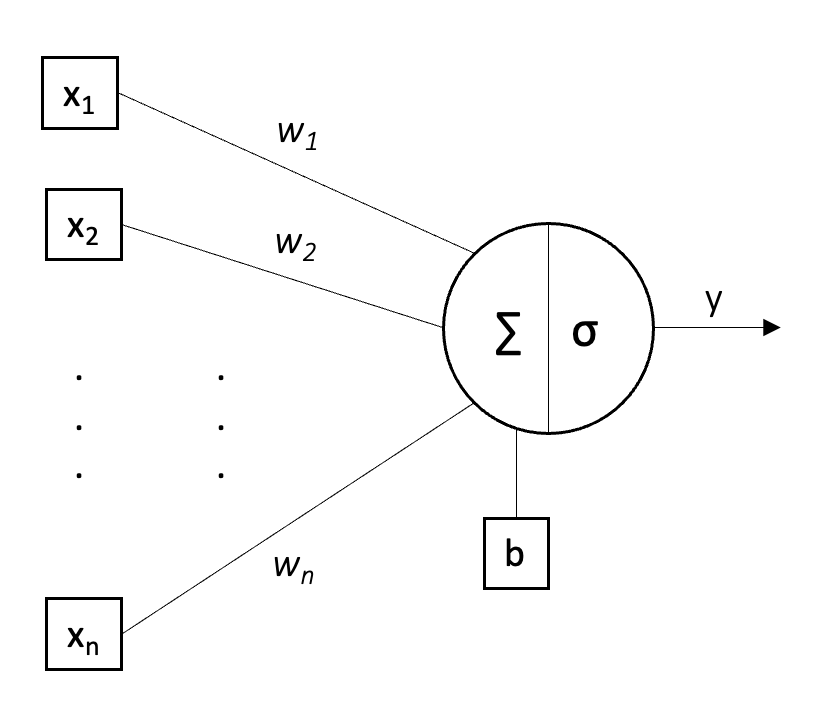
\includegraphics[scale=.4,trim={0 0.9cm 0 0},clip]{Images/single_neuron.png}
\end{figure}
Therefore, a neuron is defined by its weight vector $\mathbf{w}$, its bias $b$ and an activation function $\sigma$. $x_1, x_2, ..., x_n$ are the inputs of the neuron and y is the output. Inputs can also be seen as a vector $\mathbf{x}$.

The output of the neuron is computed as:
$$y = \sigma(\mathbf{w} \cdot \mathbf{x} + b) = \sigma(\sum_{i=0}^{n}{w_i \cdot x_i} + b)$$

In general, a neural network can have many neurons divided into many layers.
Usually, it is considered to have one input layer containing as many neurons as the number of the inputs and one output layer containing as many neurons as the dimension of the output.
Between the input and output layers, there can be one or more layers, called hidden layers.
Since we consider fully-connected neural networks every neuron of one layer is connected to all the neurons of the next layer, except for the last layer which has no outgoing arcs.
Moreover, we consider feedforward neural networks in which loops inside the structure cannot be present.

In the following, the basics of the mathematical foundations of a neural network will be given.
\begin{figure}[H]
    \centering
    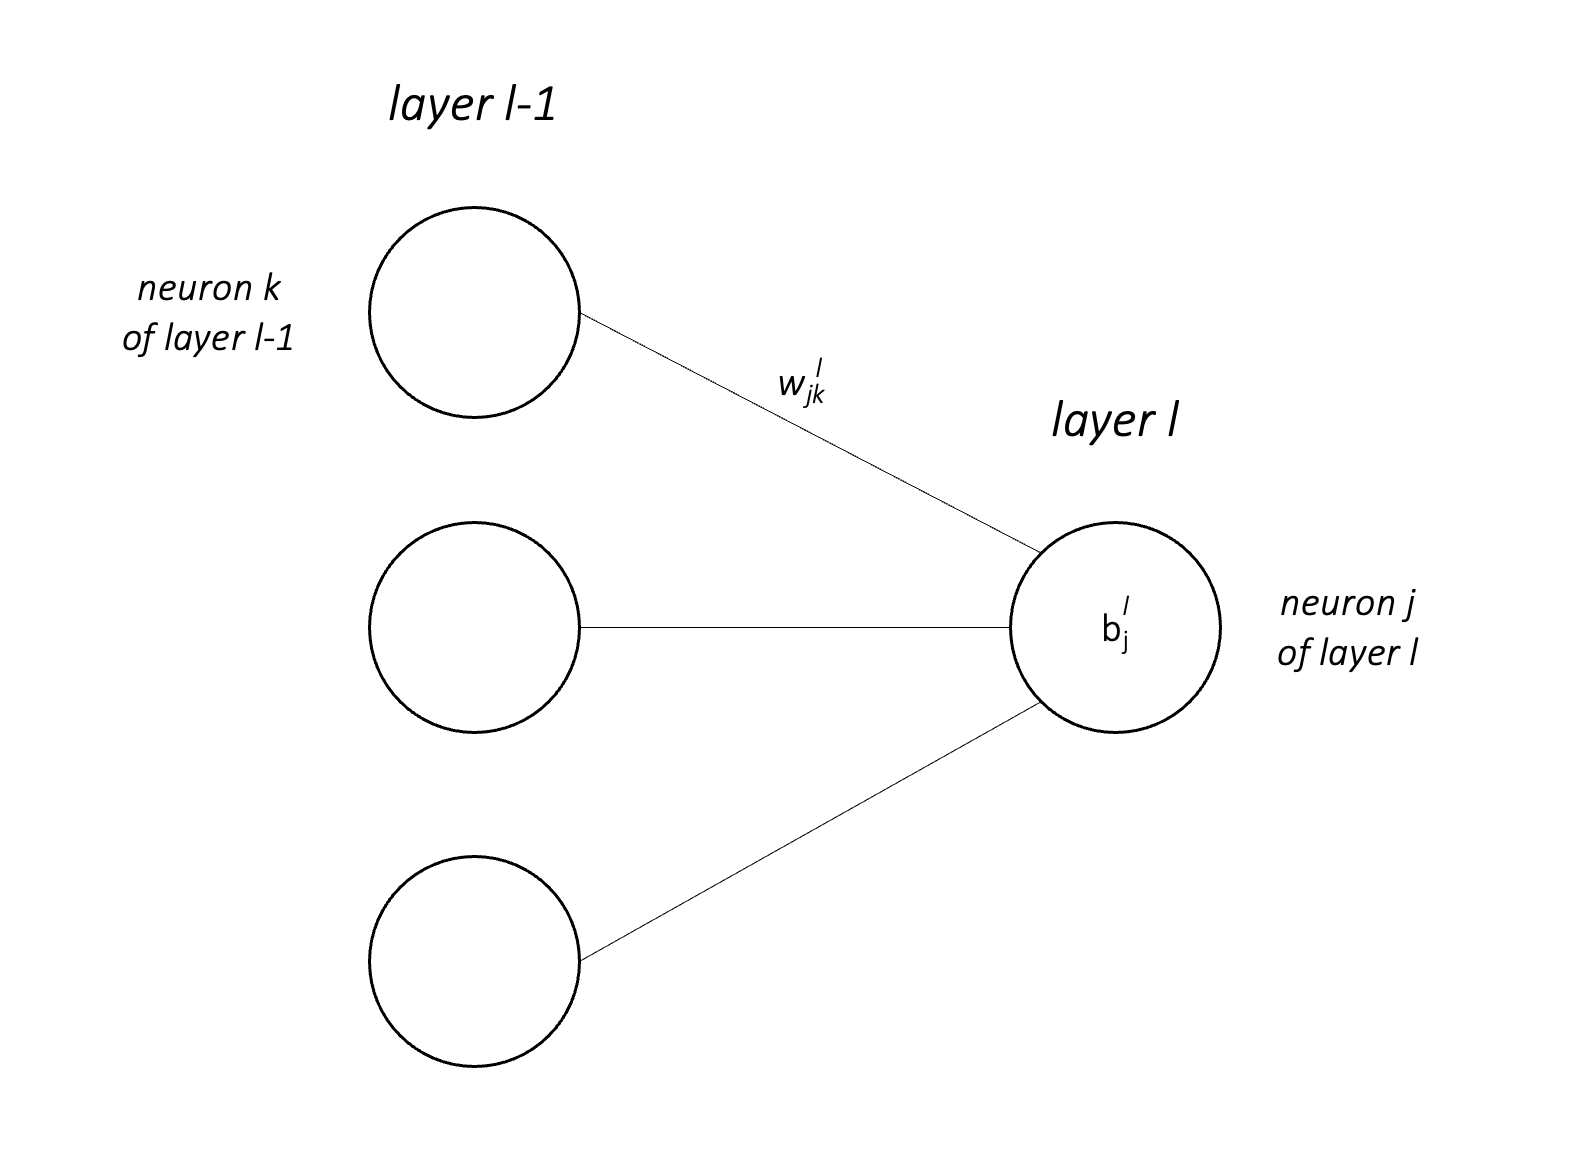
\includegraphics[scale=.3]{Images/layers_ann.png}
\end{figure}

\begin{enumerate}
    \item $b_{j}^{l}$ bias of the neuron $j$ in layer $l$,
    
    $\mathbf{b}^{l}$ vector of the biases of layer $l$
    \item $w^{l}_{jk}$ weight of the arc connecting neuron $k$ of layer $l-1$ to neuron $j$ of layer $l$,
    
    $W^{l}$ matrix of the weights of the arcs connecting layer $l-1$ and layer $l$
    \item $a_{j}^{l}$ activation of the neuron $j$ in layer $l$
    $$a_{j}^{l} = \sigma(\sum\limits_{k=0}^{size_{l-1}-1}{w_{jk}^{l} a_{k}^{l-1} + b_{j}^{l}})$$
    with $size_{l-1}$ number of neurons of the layer $l-1$,
    
    $\mathbf{a}^{l}$ activation vector
    $$\mathbf{a}^{l}=\sigma(\mathbf{W}^{l} \cdot \mathbf{a}^{l-1} + \mathbf{b}^{l})$$
\end{enumerate}

These operations are computed for each layer from the input layer until the last layer, generating the output of the network.

Artificial neural networks are used for approximating a wide range of functions thanks to the theoretical results given by the universal approximation theorem.

The set of parameters of the neural network, namely the matrices of the weights and the vectors of the biases for each layer, is created by the function \verb|initialize_parameters()| which takes as input the sizes, in terms of number of neurons, of each layer.
This function also initializes the parameters: for the weights, it is adopted a random initialization with the values sampled from a standard Gaussian distribution; the biases instead are initialized to zero.

The computation done by the artificial neural network in our code is provided by the function \verb|ANN()|, which takes as arguments the input of the neural network and its parameters and returns the output of the calculation.

Let's consider the classification of fraudulent transactions, the problem is solved as a supervised learning problem, with an ANN.
It is given a set of transactions with their features and labelled as fraud or not fraud. The input of the artificial neural network is composed of the features of a transaction and on the output it gives the class to which the transaction belongs, or better, the probability to belong to a class.
The problem of determining the mapping between the features and the class coincides, in the ANN case, to determine the values of the parameters that allow the best classification.

As in the other previously discussed classification methods, also in this one, the dataset is split into three parts, training set, validation set and test set.

\subsection{Cost functions}

The computation of the correct set of parameters is done through the solution of a minimization problem of a function that gives the measure of the discrepancy between the predictions and the correct labels. This function is called cost function.

Considering $n_{samples}$ the number of samples used as input, the cost functions we defined in the code are:
\begin{enumerate}
    \item \textbf{Cross entropy for a binary classification problem}
    $$J(\textbf{W}, \textbf{b}) = -\frac{1}{n_{samples}}\sum_{i=0}^{n_{samples}-1}{\alpha y(\mathbf{x}_i)\log{a_i^L}+\beta(1-y(\mathbf{x}_i))\log{(1-a_i^L)}}$$
    With $y(\mathbf{x}_{i})$ true label and $a_i^L$ the computed prediction, considering $L$ the last layer of the neural network. $\alpha$ and $\beta$ are weights that give more or less importance to the error made in predicting a fraudulent transaction or a not fraudulent one.
    We define this cost function inside the Python function \verb|cross_entropy()|.
    \item \textbf{Cross entropy for a general classification problem}
    $$J(\textbf{W}, \textbf{b}) = -\frac{1}{n_{samples}}\sum_{i=0}^{n_{samples}-1}{\sum_{j=0}^{n_{outputs}-1}{\alpha_{j} y_{j}(\mathbf{x}_{i})\log{a_{ji}^{L}}}}$$

    With $\mathbf{y}(\mathbf{x}_{i})$ true label (one-hot representation) and $\mathbf{a}_i^L$ the computed prediction, considering $L$ the last layer of the neural network. $\alpha_{j}$ are weights that give more or less importance to the error made in predicting a fraudulent transaction or a not fraudulent one. We define this cost function inside the Python function \verb|cross_entropy_general()|.
    \item \textbf{Mean squared error}
    $$J(\textbf{W}, \textbf{b}) = \frac{1}{n_{samples}}\sum_{i=0}^{n_{samples}-1}{\frac{1}{2} \Vert y(\mathbf{x}_i)-a_i^L\Vert^2}$$
    
    With $y(\mathbf{x}_{i})$ true label and $a_i^L$ the computed prediction, considering $L$ the last layer of the neural network
    We define this cost function inside the Python function \verb|MSE()|.
    \item \textbf{Accuracy}
    
    Is the percentage of correctly classified samples.
    We define this cost function inside the Python function \verb|accuracy()|.
\end{enumerate}

\subsection{Optimization methods}
In order to minimize the cost function with respect to the parameters, since the parameters are a lot, an iterative method is the only solution. The procedure of applying the minimization method for finding the best approximation of the mapping between input and outputs is called training of the neural network.
The following methods find their basics in the idea of updating the parameters in the inverse gradient direction in order to go in the direction that locally minimizes the cost function.
The methods we used for finding the parameters that minimize the cost function are:
\begin{enumerate}
    \item \textbf{Stochastic gradient descent (SGD)}
    
    Here we consider the stochastic gradient descent with mini-batch and adaptive learning rate, depending on the epoch of execution $k$.
    The recursive update of the parameter in the method is:
    
    $$\mathbf{g}(\mathbf{x}^{(k)})=\frac{1}{|I_{k}|}\sum_{i_k \in I_k}{\nabla J_{i_{k}}(\mathbf{x}^{(k)})}$$
    $$\mathbf{x}^{(k+1)} = \mathbf{x}^{(k)}-\gamma^{(k)} \mathbf{g}(\mathbf{x}^{(k)})$$

    with $I_{k}$ set of randomly extracted indexes of samples and with the gradient computed with respect to the weights and biases of the network, these ones contained in the variable $\mathbf{x}$. Our implementation of the method is the function \verb|SGD()|.
    
    \item \textbf{Nesterov acceleration method (NAG)}
    
    This method is similar to the stochastic gradient descent but at each iteration, the update is done taking into account the sum of the previous directions of the gradient.
    Here we consider the Nesterov acceleration method with mini-batch and adaptive learning rate, depending on the epoch of execution $k$.
    The recursive update of the parameter in the method is:
    
    $$\mathbf{v}^{(k)} = \alpha \mathbf{v}^{(k-1)}+\gamma^{(k)} \frac{1}{|I_{k}|}\sum_{i_k \in I_k}{\nabla J_{i_{k}}(\mathbf{x}^{(k)}-\alpha \mathbf{v}^{(k-1)})}$$
    $$\mathbf{x}^{(k+1)} = \mathbf{x}^{(k)}-\mathbf{v}^{(k)}$$
    
    with $I_{k}$ set of randomly extracted indexes of samples and with the gradient computed with respect to the weights and biases of the network, these ones contained in the variable $\mathbf{x}$.
    Our implementation of the method is the function \verb|NAG()|.
    \item \textbf{RMSprop}
    
    Also, this method works on the top of the stochastic gradient descent but at each iteration, the update is done taking into account the weighted sum of the previous gradients squared. In this way, the learning rate is automatically updated during execution.
    The recursive update of the parameter in the method is:

    $$\mathbf{g}(\mathbf{x}^{(k)})=\frac{1}{|I_{k}|}\sum_{i_k \in I_k}{\nabla J_{i_{k}}(\mathbf{x}^{(k)})}$$
    
    $$\mathbf{r}^{(k+1)} = \rho \mathbf{r}^{(k)} + (1 - \rho) \mathbf{g}(\mathbf{x}^{(k)}) \odot \mathbf{g}(\mathbf{x}^{(k)})$$
    
    $$\boldsymbol{\theta}^{(k+1)} = \boldsymbol{\theta}^{(k)} - \frac{\lambda}{\delta + \sqrt{\mathbf{r}^{(k+1)}}} \odot \mathbf{g}(\mathbf{x}^{(k)})$$
    
    with $I_{k}$ set of randomly extracted indexes of samples and with the gradient computed with respect to the weights and biases of the network, these ones contained in the variable $\mathbf{x}$. $\rho$ is the rate of decay of the history of the gradients since past values of the gradient become less important when time passes, $\delta$ is a parameter used to avoid division by zero and $\lambda$ is a sort of initial value for the learning rate.
    Our implementation of the method is the function \verb|RMSprop()|.
\end{enumerate}

The learning rate $\gamma^{(k)}$ is computed using a linear decay, already explained in the logistic regression classifier:
$$\gamma^{(k)} = \max\left(\gamma_{\min}, \gamma_{\max} (1 - \frac{k}{K})\right)$$

where $k$ is the number of the current epoch and $K$ is the number of epochs to reach $\lambda_{\min}$.

Within the optimization methods the gradients are computed using the automatic differentiation library \verb|JAX|. \verb|JAX| is also used for speeding up the code through the just-in-time compilation of the functions.

The chosen minimization method is applied to the neural network using as input the data contained in the training set.

During the training phase, the loss function has been computed also on the validation set in order to evaluate whether the model of the neural network is generalizing in a good way the input-output mapping.

The history of training, namely the values assumed by the cost function during the training step are stored, by means of the function \verb|dump()|, and then plotted by the function \verb|plot_history()|. \verb|dump()| computes the values of the different cost functions in order to make a comparison between them possible. For speeding up the computations some cost function computations can be commented.

\subsection{Regularization}
In order to evaluate if a better result can be achieved we also use a regularization method, implemented through the functions \verb|MSW()| and the \verb|cost_regularization()|. This function is used as a cost function in the training phase in order to penalize neural networks with big weights since they are a symptom of overfitting.
The mean square weight is defined as:
$$\mathrm{MSW}(\textbf{W}) = \frac{1}{n_{weights}} \sum_{i=1}^{n_{weights}} w_i^2$$
Therefore the new cost function will be:
$$J_{regularization}(\textbf{W}, \textbf{b}) = J(\textbf{W}, \textbf{b}) + \beta \,\mathrm{MSW}(\textbf{W})$$

where $\beta$ is the regularization parameter.

\subsection{Implementation choices and parameters}
We choose to implement two slightly different neural networks: one with one scalar output representing the probability of the input vector to represent a fraudulent transaction and one with two scalar outputs  representing the probability of the input vector to represent a fraudulent transaction and to represent a not fraudulent transaction respectively.

The implementation choices we adopted for the first neural network are the following:
\begin{enumerate}
    \item Activation function of the neural network: 
    \begin{itemize}
        \item\textbf{hyperbolic tangent} on all the layers except for the last one
        \item\textbf{sigmoid} on the last layer
    \end{itemize}
    \item Cost function: \textbf{cross entropy for a binary classification problem with regularization}
    \item Weights for the class losses: \textbf{[2.8, 1]}
    \item Layers size: \textbf{[input size, 30, 20, 1]}
    \item Optimization method: \textbf{RMSprop}
    \begin{itemize}
        \item Number of epochs: \textbf{2000}
        \item Mini-batch size: \textbf{256}
    \end{itemize}
    \item \textbf{Small regularization weight}
\end{enumerate}

The implementation choices we adopted for the second neural network are the following:
\begin{enumerate}
    \item Activation function of the neural network: 
    \begin{itemize}
        \item\textbf{hyperbolic tangent} on all the layers except for the last one
        \item\textbf{softmax} on the last layer
    \end{itemize}
    \item Cost function: \textbf{cross entropy for a general classification problem with regularization}
    \item Weights for the class losses: \textbf{[3.2, 1]}
    \item Layers size: \textbf{[input size, 30, 30, 10, 2]}
    \item Optimization method: \textbf{RMSprop}
        \begin{itemize}
        \item Number of epochs: \textbf{2500}
        \item Mini-batch size: \textbf{256}
    \end{itemize}
    \item \textbf{Small regularization weight}
\end{enumerate}

The set of hyperparameters and the type of design we chose has been driven by some heuristics and consideration but is also the result of many trials in guessing their best values. The set of parameters we found allows the neural network to reach good results in terms of the principal metrics we adopted. Modifying the parameters slightly better results might be found.

In the end, we decided to use as activation function \verb|tanh| since only a few parameters were needed and not too many epochs were required to find a good model.

Although we tried other optimization methods, RMSprop was the best one in terms of results, requiring fewer epochs but a higher number of samples in the mini-batch. In the other methods, the tuning of the parameters was more difficult.

Regularization is not too useful in this case. Too high penalization makes higher the precision but lowers a lot the recall until making too small the weights.
We use the small value of the penalization in order to avoid overfitting, it is not necessary but increases a bit the results.

\chapter{Metrics}
In order to compare the results with the aforementioned paper, we decided to use the same performance metrics. In this context of card fraud detection, the aim is to classify accurately the fraudulent transactions using a binary classifier, so we define:
\begin{itemize}
    \item true positive (TP) as the number of frauds correctly classified as frauds;
    \item true negative (TN) as the number of normal transactions correctly classified as normal;
    \item false positive (FP) as the number of normal transactions wrongly classified as frauds;
    \item false negative (FN) as the number of frauds wrongly classified as normal transactions.
\end{itemize}

Using these values the adopted metrics are:
\begin{itemize}
    \item accuracy (AC) that is the percentage of accurately classified transactions, fraudulent and not fraudulent;
    \item recall (RC) that tells how many transactions are accurately classified as frauds on the total of fraudulent transactions;
    \item precision (PR) that tells how many transactions are accurately classified as frauds on the total of transactions that are classified as frauds;
    \item F1-Score (F1) that is a measure of the correctness of the classification based on RC and PR.
\end{itemize}

Expressing the metrics using their formulas:
$$AC = \frac{TN + TP}{TP + TN + FP + FN}$$
$$RC = \frac{TP}{FN + TP}$$
$$PR = \frac{TP}{FP + TP}$$
$$F1_{score} = 2 \cdot \frac{PR \cdot RC}{PR + RC}$$

To compute all these values we implemented the function \verb|metrics()|.

During the training phase, we noticed that by changing some hyperparameters it is possible to raise some values of these metrics to the detriment of others. Hence, the optimal values depend on what the research is focused on. 

We computed also the receiver operating characteristic (ROC) curve that allows visualizing the performance of a model at different thresholds, with the associated area under the ROC curve (AUC).
The range of values of AUC is between 0 and 1 and the higher the value of AUC, the better the classification model.

\chapter{Results}
In this chapter, we report the results obtained with each classifier grouped by the datasets associated with the selected feature vectors. For each dataset, we show:
\begin{itemize}
    \item a bar plot with the values of accuracy, recall, precision and F1-score obtained by every classifier on the test set;
    \item a table with the comparison of the previous values with respect to the ones obtained in the reference paper, which are shown in grey;
    \item ROC curve for each classifier with the associated value of the AUC.
\end{itemize}
In addition to the five datasets, also the full feature vector (dataset 6) and the feature vector generated with a random approach (dataset 7) are considered.

\verb|ANN1| refers to the ANN with one output, instead \verb|ANN2| to the ANN with 2 outputs.
\begin{figure}[H]
\centering
\begin{subfigure}
    \centering
    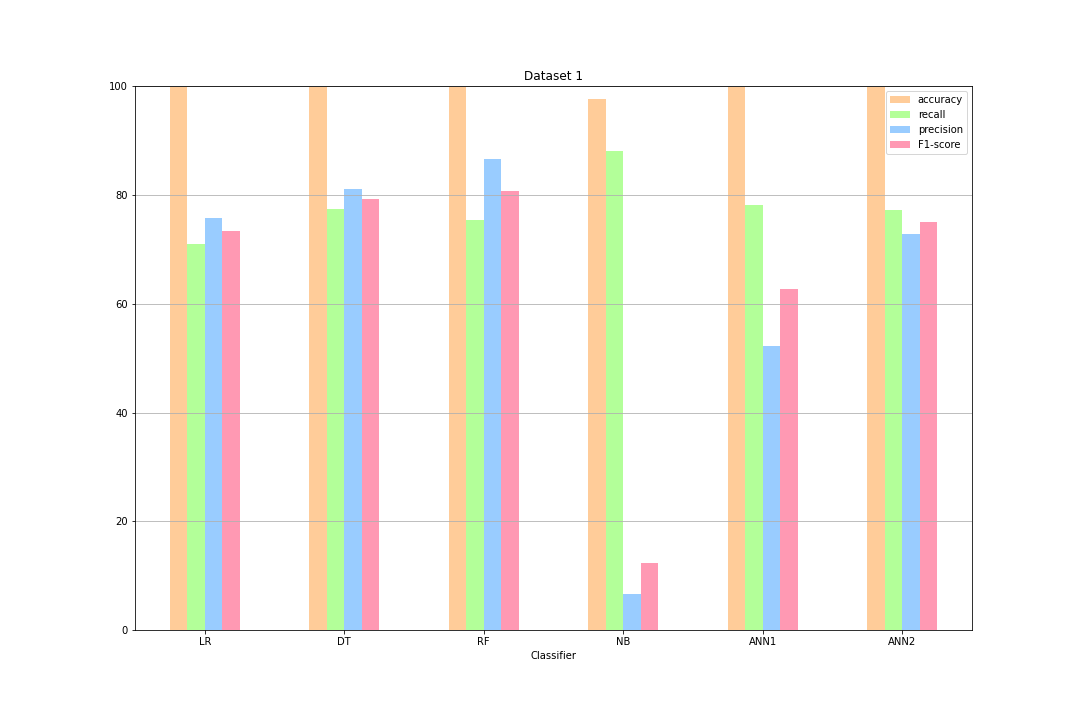
\includegraphics[scale=0.3]{Images/Dataset_1.png}
\end{subfigure}
% dataset 1
\renewcommand{\arraystretch}{0.8}% Tighter
\begin{table}[H]
\centering 
    \begin{tabular}{ c  c  c  c  c }
    \hline 
    \textbf{Model}  & \textbf{Accuracy} & \textbf{Recall} & \textbf{Precision} & \textbf{F1-Score} \\
    \hline
    RF	& 99.93	& 75.48	& 86.67 & 80.69 \\
        & \footnotesize\textcolor{gray}{99.94} & \footnotesize\textcolor{gray}{76.99} & \footnotesize\textcolor{gray}{89.69} & \footnotesize\textcolor{gray}{82.85} \\[0.01cm]
    DT	& 99.93	& 77.42	& 81.08 & 79.21 \\
        & \footnotesize\textcolor{gray}{99.92} & \footnotesize\textcolor{gray}{75.22} & \footnotesize\textcolor{gray}{75.22} & \footnotesize\textcolor{gray}{75.22} \\
    ANN1 & 99.83 & 78.22 & 52.32 & 62.70 \\
    ANN2 & 99.91 & 77.23 & 72.90 & 75.00 \\
         & \footnotesize\textcolor{gray}{99.94} & \footnotesize\textcolor{gray}{77.87} & \footnotesize\textcolor{gray}{84.61} & \footnotesize\textcolor{gray}{81.10} \\
    NB	& 97.77	& 88.12	& 6.62 & 12.31 \\
        & \footnotesize\textcolor{gray}{98.13} & \footnotesize\textcolor{gray}{84.95} & \footnotesize\textcolor{gray}{6.83} & \footnotesize\textcolor{gray}{12.65} \\
    LR	& 99.91	& 70.97	& 75.86 & 73.33 \\
        & \footnotesize\textcolor{gray}{99.91} & \footnotesize\textcolor{gray}{57.52} & \footnotesize\textcolor{gray}{82.27} & \footnotesize\textcolor{gray}{67.70} \\
    \hline
    \end{tabular}
\end{table}
\begin{subfigure}
    \centering
    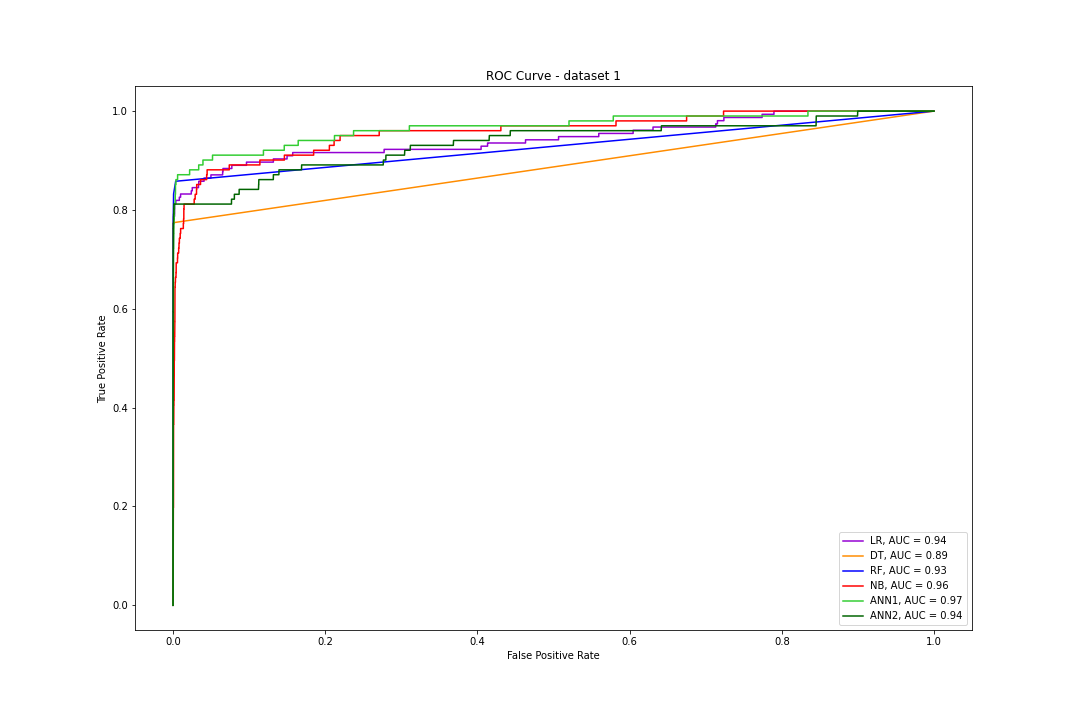
\includegraphics[scale=0.3]{Images/ROC_1.png}
\end{subfigure}
  \caption{Results for dataset 1.}
\end{figure}



\begin{figure}[H]
\centering
\begin{subfigure}
    \centering
    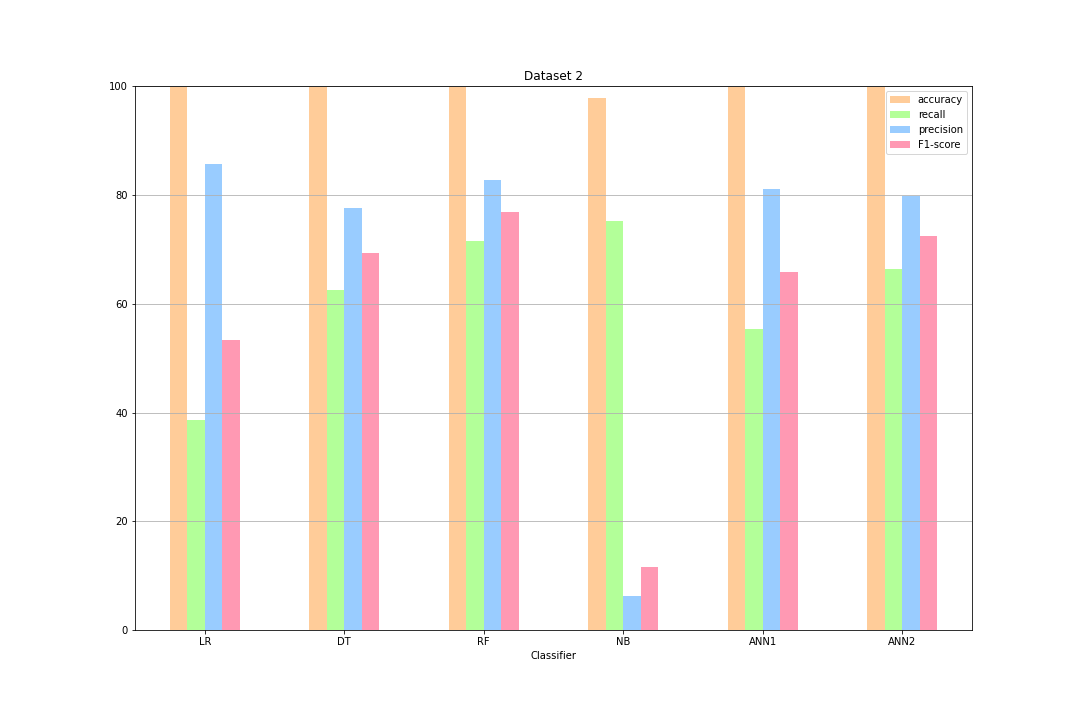
\includegraphics[scale=0.3]{Images/Dataset_2.png}
\end{subfigure}

% dataset 2
\renewcommand{\arraystretch}{0.8}% Tighter
\begin{table}[H]
\centering 
    \begin{tabular}{ c  c  c  c  c }
    \hline 
    \textbf{Model}  & \textbf{Accuracy} & \textbf{Recall} & \textbf{Precision} & \textbf{F1-Score} \\
    \hline
    RF	& 99.92 & 71.61	& 82.84 & 76.82 \\
        & \footnotesize\textcolor{gray}{99.93} & \footnotesize\textcolor{gray}{76.10} & \footnotesize\textcolor{gray}{82.69} & \footnotesize\textcolor{gray}{79.26} \\[0.01cm]
    DT	& 99.90 & 62.58	& 77.60 & 69.29 \\
        & \footnotesize\textcolor{gray}{99.87} & \footnotesize\textcolor{gray}{68.14} & \footnotesize\textcolor{gray}{60.62} & \footnotesize\textcolor{gray}{64.16} \\
    ANN1 & 99.90 & 55.45 & 81.16 & 65.88 \\
    ANN2 & 99.91 & 66.34 & 79.76 & 72.43 \\
         & \footnotesize\textcolor{gray}{99.91} & \footnotesize\textcolor{gray}{66.37} & \footnotesize\textcolor{gray}{76.53} & \footnotesize\textcolor{gray}{71.09} \\
    NB	& 97.95 & 75.25	& 6.25 & 11.54 \\
        & \footnotesize\textcolor{gray}{98.65} & \footnotesize\textcolor{gray}{77.87} & \footnotesize\textcolor{gray}{8.59} & \footnotesize\textcolor{gray}{15.47} \\
    LR	& 99.88 & 38.71	& 85.71 & 53.33 \\
        & \footnotesize\textcolor{gray}{99.89} & \footnotesize\textcolor{gray}{47.78} & \footnotesize\textcolor{gray}{79.41} & \footnotesize\textcolor{gray}{59.66} \\
    \hline
    \end{tabular}
\end{table}

\begin{subfigure}
    \centering
    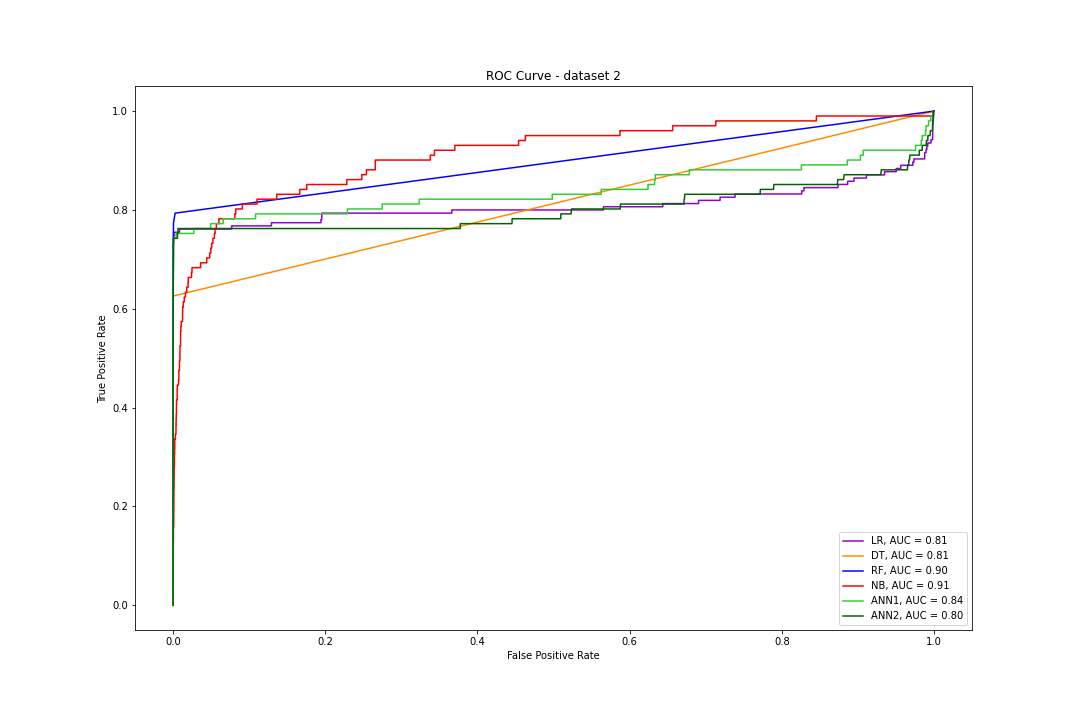
\includegraphics[scale=0.3]{Images/ROC_2.png}
\end{subfigure}
  \caption{Results for dataset 2.}
\end{figure}



\begin{figure}[H]
\centering
\begin{subfigure}
    \centering
    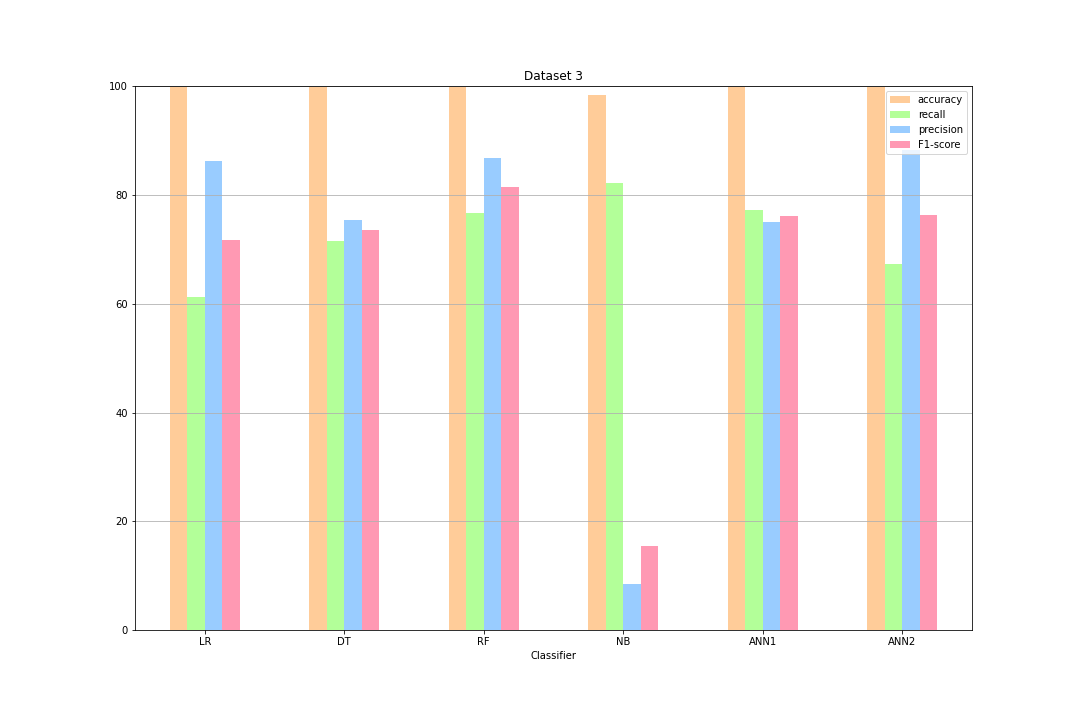
\includegraphics[scale=0.3]{Images/Dataset_3.png}
\end{subfigure}

% dataset 3
\renewcommand{\arraystretch}{0.8}% Tighter
\begin{table}[H]
\centering 
    \begin{tabular}{ c  c  c  c  c }
    \hline 
    \textbf{Model}  & \textbf{Accuracy} & \textbf{Recall} & \textbf{Precision} & \textbf{F1-Score} \\
    \hline
    RF	& 99.94 &	76.77 &	86.86 &	81.51 \\
        & \footnotesize\textcolor{gray}{99.94} & \footnotesize\textcolor{gray}{75.22} & \footnotesize\textcolor{gray}{85.85} & \footnotesize\textcolor{gray}{80.18} \\[0.01cm]
    DT	& 99.91 &	71.61 &	75.51 &	73.51 \\
        & \footnotesize\textcolor{gray}{99.90} & \footnotesize\textcolor{gray}{76.10} & \footnotesize\textcolor{gray}{68.80} & \footnotesize\textcolor{gray}{72.26} \\
    ANN1 & 99.91 & 77.23 & 75.00 & 76.10 \\
    ANN2 & 99.93 & 67.33 & 88.31 & 76.40 \\
         & \footnotesize\textcolor{gray}{99.91} & \footnotesize\textcolor{gray}{67.25} & \footnotesize\textcolor{gray}{77.55} & \footnotesize\textcolor{gray}{72.03} \\
    NB	& 98.40 &	82.18 &	8.49 &	15.38 \\
        & \footnotesize\textcolor{gray}{98.81} & \footnotesize\textcolor{gray}{81.41} & \footnotesize\textcolor{gray}{10.07} & \footnotesize\textcolor{gray}{17.93} \\
    LR	& 99.91 &	61.29 &	86.36 &	71.70 \\
        & \footnotesize\textcolor{gray}{99.90} & \footnotesize\textcolor{gray}{53.09} & \footnotesize\textcolor{gray}{80.00} & \footnotesize\textcolor{gray}{63.82} \\
    \hline
    \end{tabular}
\end{table}

\begin{subfigure}
    \centering
    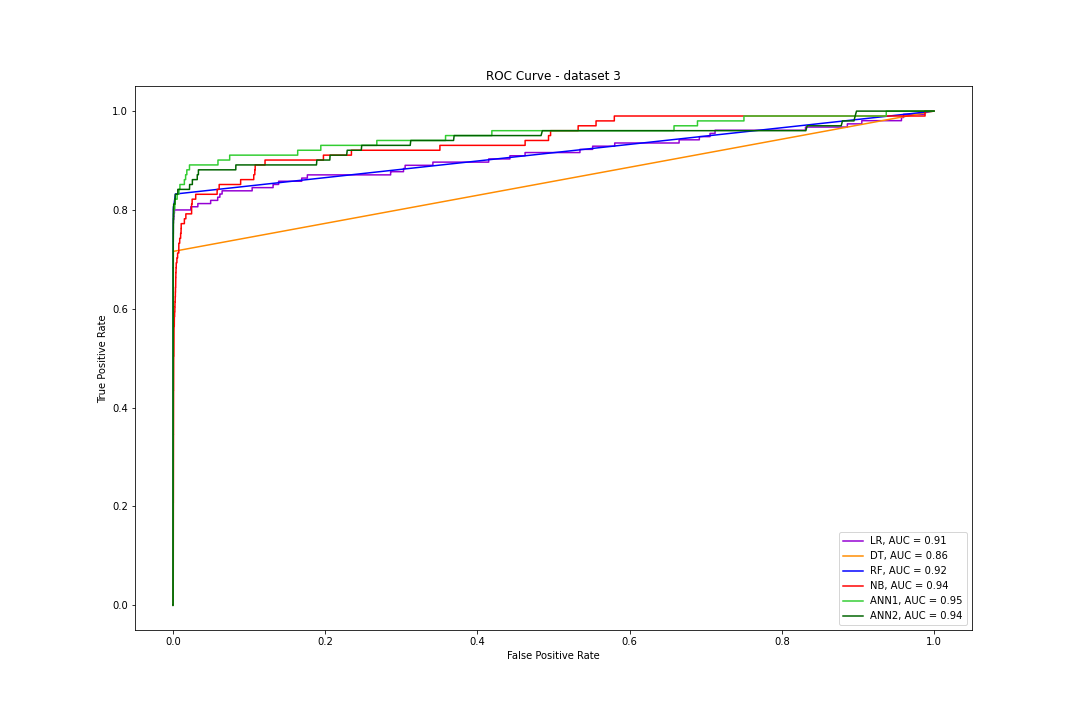
\includegraphics[scale=0.3]{Images/ROC_3.png}
\end{subfigure}
  \caption{Results for dataset 3.}
\end{figure}


\begin{figure}[H]
\centering
\begin{subfigure}
    \centering
    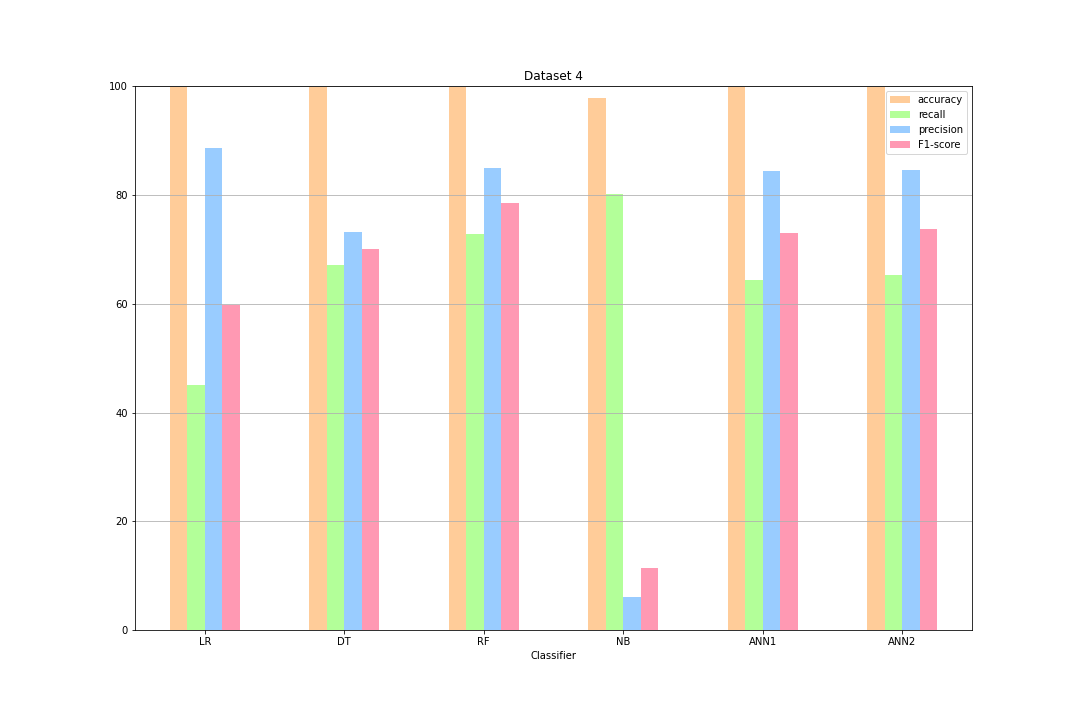
\includegraphics[scale=0.3]{Images/Dataset_4.png}
\end{subfigure}

% dataset 4
\renewcommand{\arraystretch}{0.8}% Tighter
\begin{table}[H]
\centering 
    \begin{tabular}{ c  c  c  c  c }
    \hline 
    \textbf{Model}  & \textbf{Accuracy} & \textbf{Recall} & \textbf{Precision} & \textbf{F1-Score} \\
    \hline
    RF	& 99.93 &	72.90 &	84.96 &	78.47 \\
        & \footnotesize\textcolor{gray}{99.94} & \footnotesize\textcolor{gray}{77.87} & \footnotesize\textcolor{gray}{83.80} & \footnotesize\textcolor{gray}{80.73} \\[0.01cm]
    DT	& 99.90 &	67.10 &	73.24 &	70.03 \\
        & \footnotesize\textcolor{gray}{99.91} & \footnotesize\textcolor{gray}{76.10} & \footnotesize\textcolor{gray}{72.26} & \footnotesize\textcolor{gray}{74.13} \\
    ANN1 & 99.92 & 64.36 & 84.42 & 73.03 \\
    ANN2 & 99.92 & 65.35 & 84.62 & 73.74 \\
         & \footnotesize\textcolor{gray}{99.91} & \footnotesize\textcolor{gray}{61.06} & \footnotesize\textcolor{gray}{81.17} & \footnotesize\textcolor{gray}{69.69} \\
    NB	& 97.78 &	80.20 &	6.12 &	11.38 \\
        & \footnotesize\textcolor{gray}{98.48} & \footnotesize\textcolor{gray}{81.41} & \footnotesize\textcolor{gray}{7.97} & \footnotesize\textcolor{gray}{14.53} \\
    LR	& 99.89 &	45.16 &	88.61 &	59.83 \\
        & \footnotesize\textcolor{gray}{99.89} & \footnotesize\textcolor{gray}{46.90} & \footnotesize\textcolor{gray}{77.94} & \footnotesize\textcolor{gray}{58.56} \\
    \hline
    \end{tabular}
\end{table}

\begin{subfigure}
    \centering
    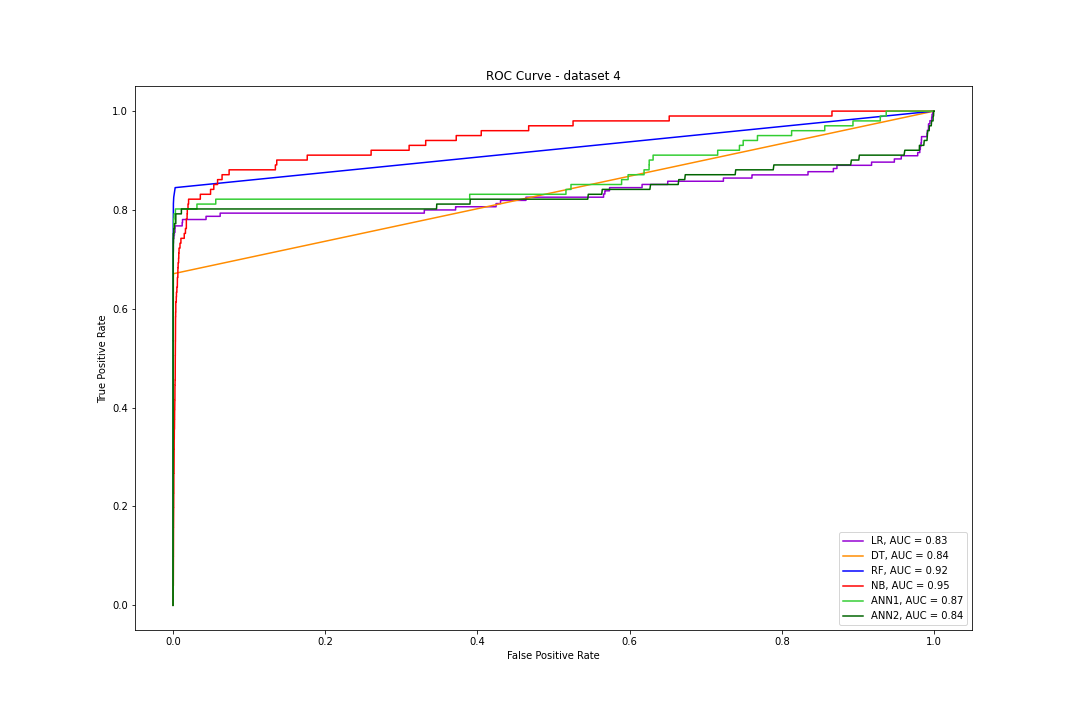
\includegraphics[scale=0.3]{Images/ROC_4.png}
\end{subfigure}
  \caption{Results for dataset 4.}
\end{figure}



\begin{figure}[H]
\centering
\begin{subfigure}
    \centering
    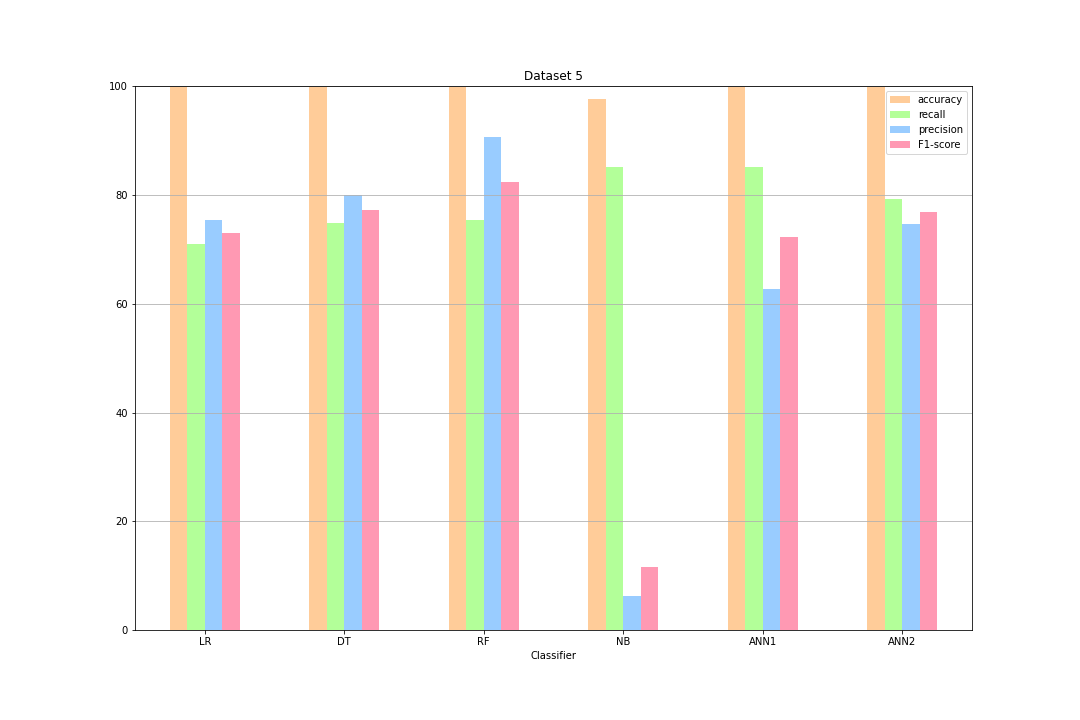
\includegraphics[scale=0.3]{Images/Dataset_5.png}
\end{subfigure}

% dataset 5
\renewcommand{\arraystretch}{0.8}% Tighter
\begin{table}[H]
\centering 
    \begin{tabular}{ c  c  c  c  c }
    \hline 
    \textbf{Model}  & \textbf{Accuracy} & \textbf{Recall} & \textbf{Precision} & \textbf{F1-Score} \\
    \hline
    RF	& 99.94 &	75.48 &	90.70 &	82.39 \\
        & \footnotesize\textcolor{gray}{99.98} & \footnotesize\textcolor{gray}{72.56} & \footnotesize\textcolor{gray}{95.34} & \footnotesize\textcolor{gray}{82.41} \\[0.01cm]
    DT	& 99.92 &	74.84 &	80.00 &	77.33 \\
        & \footnotesize\textcolor{gray}{99.89} & \footnotesize\textcolor{gray}{72.56} & \footnotesize\textcolor{gray}{65.07} & \footnotesize\textcolor{gray}{68.61} \\
    ANN1 & 99.88 & 85.15 & 62.77 & 72.27 \\
    ANN2 & 99.92 & 79.21 & 74.77 & 76.92 \\
         & \footnotesize\textcolor{gray}{99.08} & \footnotesize\textcolor{gray}{77.87} & \footnotesize\textcolor{gray}{12.27} & \footnotesize\textcolor{gray}{21.20} \\
    NB	& 97.69 &	85.15 &	6.20 &	11.57 \\
        & \footnotesize\textcolor{gray}{99.44} & \footnotesize\textcolor{gray}{57.52} & \footnotesize\textcolor{gray}{15.85} & \footnotesize\textcolor{gray}{24.85} \\
    LR	& 99.91 &	70.97 &	75.34 &	73.09 \\
        & \footnotesize\textcolor{gray}{99.77} & \footnotesize\textcolor{gray}{46.90} & \footnotesize\textcolor{gray}{34.64} & \footnotesize\textcolor{gray}{39.84} \\
    \hline
    \end{tabular}
\end{table}

\begin{subfigure}
    \centering
    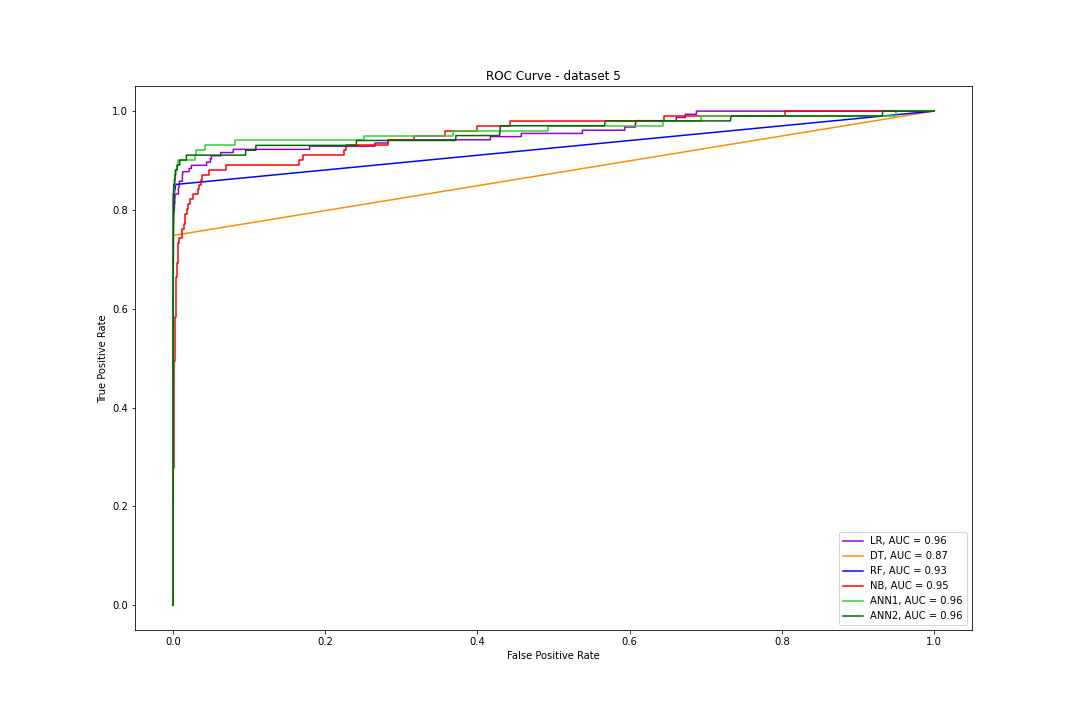
\includegraphics[scale=0.3]{Images/ROC_5.png}
\end{subfigure}
  \caption{Results for dataset 5.}
\end{figure}



\begin{figure}[H]
\centering
\begin{subfigure}
    \centering
    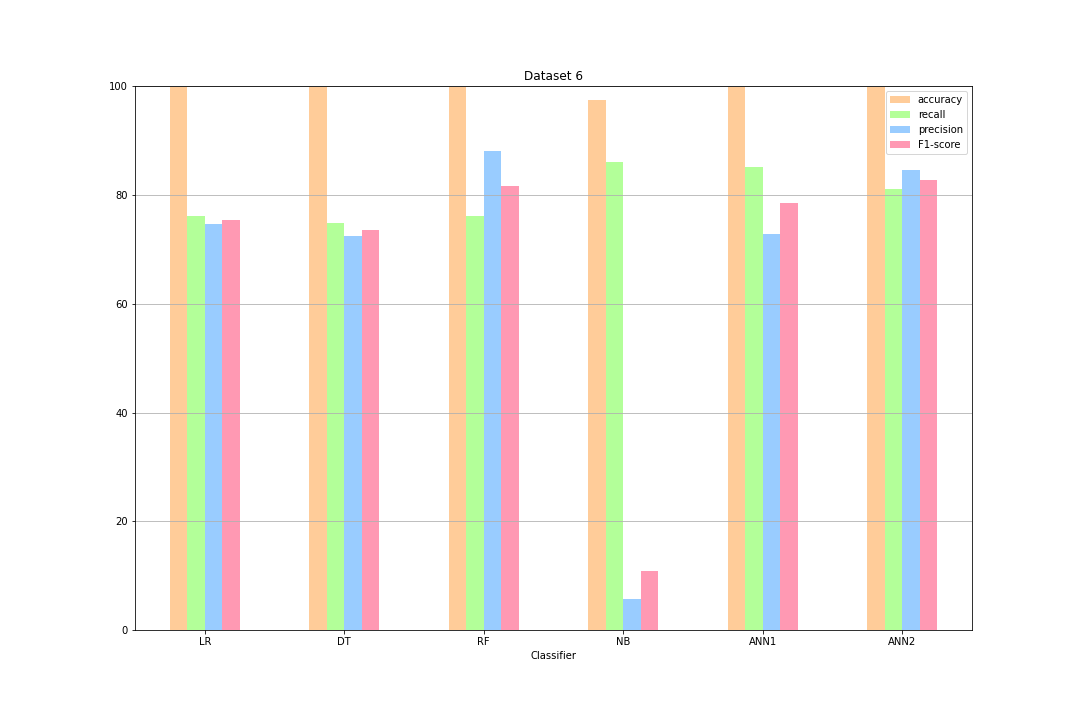
\includegraphics[scale=0.3]{Images/Dataset_6.png}
\end{subfigure}

% dataset 6
\renewcommand{\arraystretch}{0.8}% Tighter
\begin{table}[H]
\centering 
    \begin{tabular}{ c  c  c  c  c }
    \hline 
    \textbf{Model}  & \textbf{Accuracy} & \textbf{Recall} & \textbf{Precision} & \textbf{F1-Score} \\
    \hline
    RF	& 99.94 &	76.13 &	88.06 &	81.66 \\
        & \footnotesize\textcolor{gray}{87.95} & \footnotesize\textcolor{gray}{77.87} & \footnotesize\textcolor{gray}{92.63} & \footnotesize\textcolor{gray}{84.61} \\[0.01cm]
    DT	& 99.90 & 74.84 &	72.50 &	73.65 \\
        & \footnotesize\textcolor{gray}{96.91} & \footnotesize\textcolor{gray}{76.10} & \footnotesize\textcolor{gray}{71.07} & \footnotesize\textcolor{gray}{73.50} \\
    ANN1 & 99.92 & 85.15 & 72.88 & 78.54 \\
    ANN2 & 99.94 & 81.19 & 84.54 & 82.83 \\
         & \footnotesize\textcolor{gray}{97.80} & \footnotesize\textcolor{gray}{74.33} & \footnotesize\textcolor{gray}{42.85} & \footnotesize\textcolor{gray}{54.36} \\
    NB	& 97.49 &	86.14 &	5.78 &	10.83 \\
        & \footnotesize\textcolor{gray}{80.31} & \footnotesize\textcolor{gray}{64.60} & \footnotesize\textcolor{gray}{13.95} & \footnotesize\textcolor{gray}{22.95} \\
    LR	& 99.91 &	76.13 &	74.68 &	75.40 \\
        & \footnotesize\textcolor{gray}{93.88} & \footnotesize\textcolor{gray}{60.17} & \footnotesize\textcolor{gray}{62.96} & \footnotesize\textcolor{gray}{61.53} \\
    \hline
    \end{tabular}
\end{table}

\begin{subfigure}
    \centering
    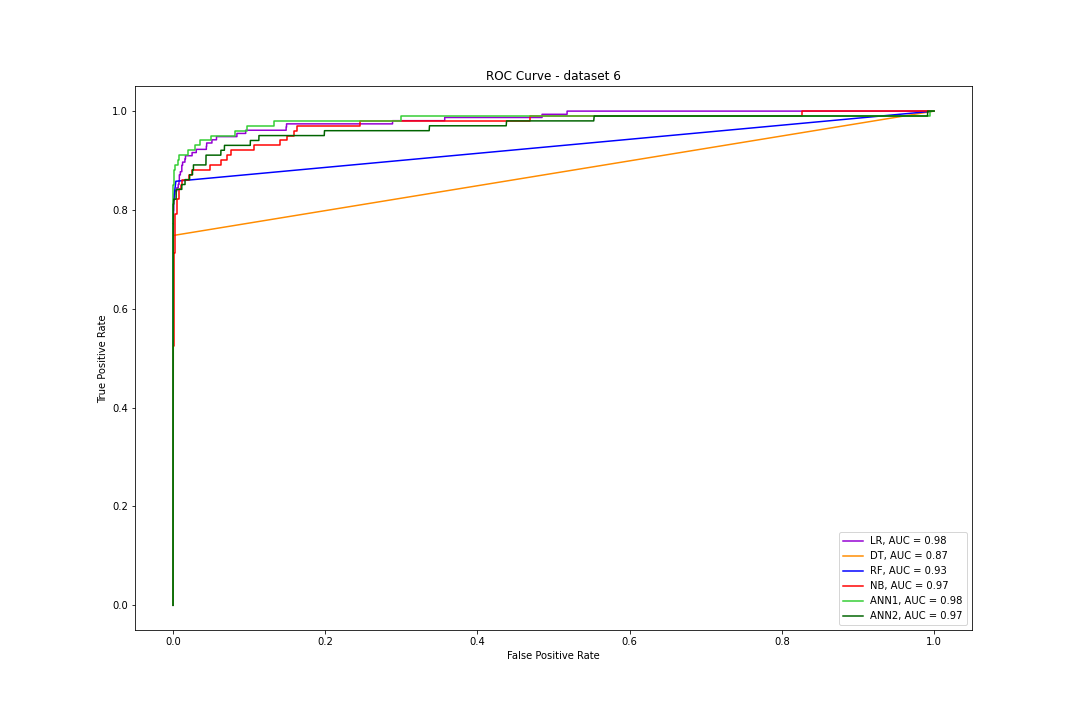
\includegraphics[scale=0.3]{Images/ROC_6.png}
\end{subfigure}
  \caption{Results for dataset 6.}
\end{figure}



\begin{figure}[H]
\centering
\begin{subfigure}
    \centering
    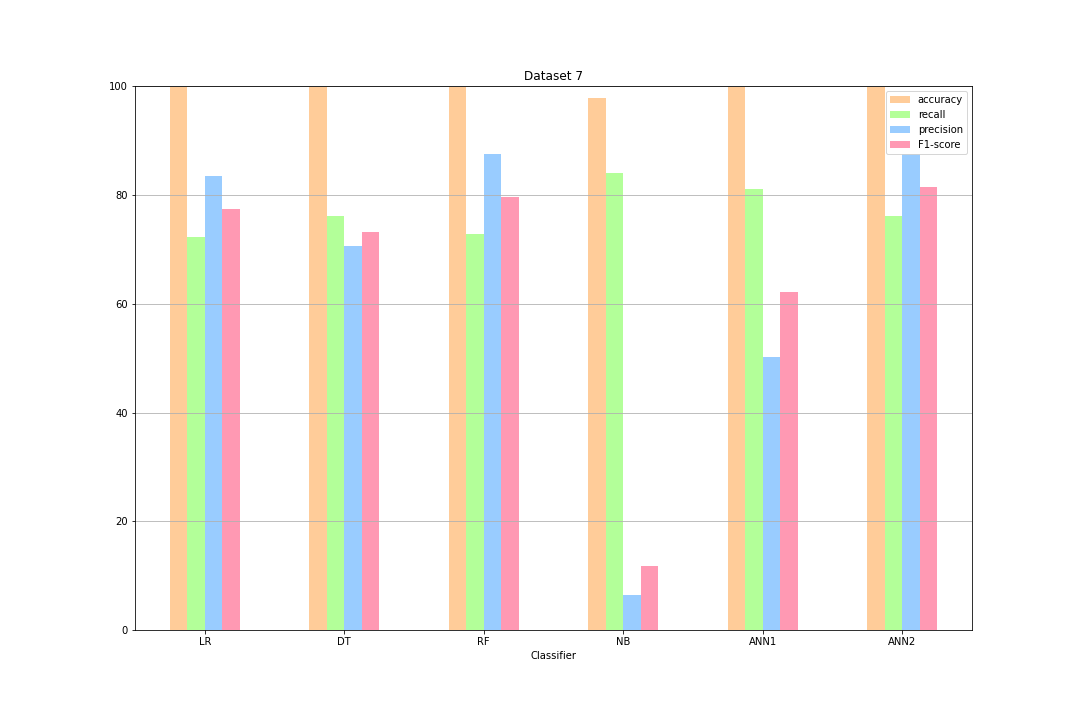
\includegraphics[scale=0.3]{Images/Dataset_7.png}
\end{subfigure}

% dataset 7
\renewcommand{\arraystretch}{0.8}% Tighter
\begin{table}[H]
\centering 
    \begin{tabular}{ c  c  c  c  c }
    \hline 
    \textbf{Model}  & \textbf{Accuracy} & \textbf{Recall} & \textbf{Precision} & \textbf{F1-Score} \\
    \hline
    RF	& 99.93 &	72.90 &	87.60 &	79.58 \\
        & \footnotesize\textcolor{gray}{83.78} & \footnotesize\textcolor{gray}{79.64} & \footnotesize\textcolor{gray}{92.78} & \footnotesize\textcolor{gray}{85.71} \\[0.01cm]
    DT	& 99.90 &	76.13 &	70.66 &	73.29 \\
        & \footnotesize\textcolor{gray}{89.91} & \footnotesize\textcolor{gray}{79.64} & \footnotesize\textcolor{gray}{68.70} & \footnotesize\textcolor{gray}{73.77} \\
    ANN1 & 99.82 & 81.19 & 50.31 & 62.12 \\
    ANN2 & 99.94 & 76.24 & 87.50 & 81.48 \\
         & \footnotesize\textcolor{gray}{88.93} & \footnotesize\textcolor{gray}{78.76} & \footnotesize\textcolor{gray}{82.40} & \footnotesize\textcolor{gray}{80.54} \\
    NB	& 97.78 &	84.16 &	6.37 &	11.85 \\
        & \footnotesize\textcolor{gray}{78.14} & \footnotesize\textcolor{gray}{83.18} & \footnotesize\textcolor{gray}{6.73} & \footnotesize\textcolor{gray}{12.46} \\
    LR	& 99.92 & 72.26 &	83.58 &	77.51 \\
        & \footnotesize\textcolor{gray}{79.91} & \footnotesize\textcolor{gray}{59.29} & \footnotesize\textcolor{gray}{81.70} & \footnotesize\textcolor{gray}{68.71} \\
    \hline
    \end{tabular}
\end{table}

\begin{subfigure}
    \centering
    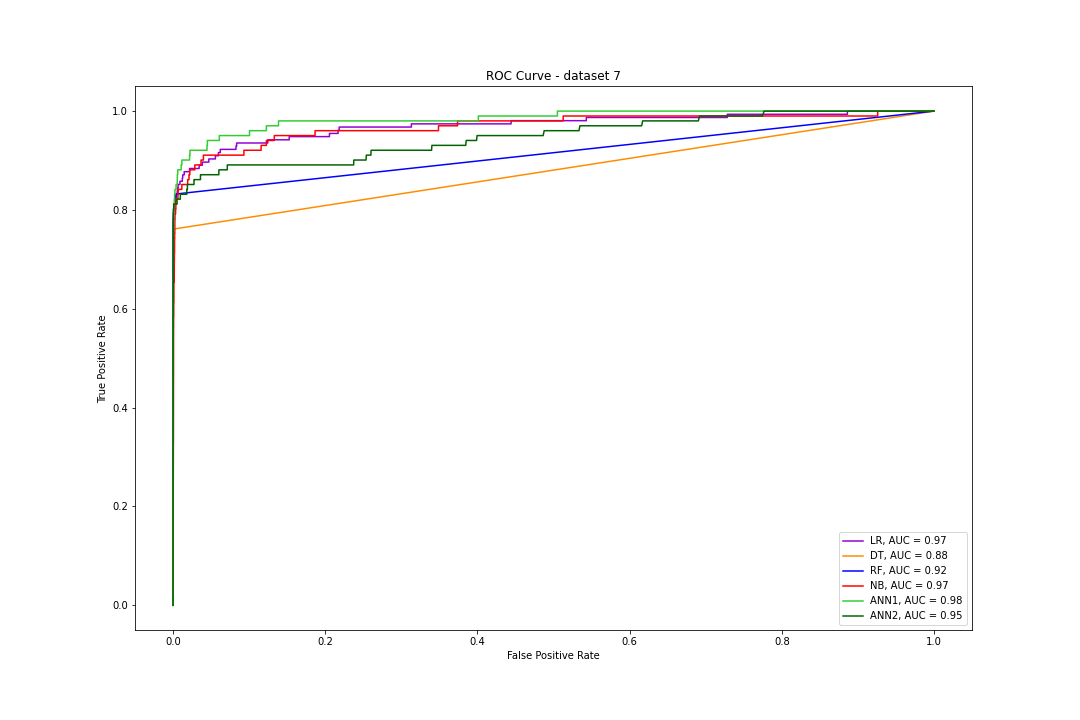
\includegraphics[scale=0.3]{Images/ROC_7.png}
\end{subfigure}
  \caption{Results for dataset 7.}
\end{figure}



\chapter{Conclusion}
In the first five datasets, which use the GA-selected features, we found good values of all the metrics, comparable with the ones pointed out by the scientific paper.
In the last two datasets, namely the entire one and the one with randomly selected features, we did not notice a significant drop in accuracy like the one highlighted in the paper.
We end up saying that the selection of the features using GA does not improve so much the goodness of the generated models but we agree that the methods are faster in terms of execution time since we use a smaller amount of data.

In general, the accuracy is around 99.9\%, only naive Bayes models struggle to reach this threshold and have an average accuracy of 98\%.
Overall naive Bayes didn't perform well since we can only optimize the model for having a high recall or a high precision but not both. It's evident from the bar plots that this model has problems fitting the underlying structure of the data. 
Concerning the other models it is true that RF performs almost always better than DT, but it requires also more memory and training time than DT. DT seems to be a good compromise among all the datasets since it takes little time to train, has just a few hyperparameters to tune and can create simpler models.
Considering the ANN, instead, it reaches good performances but it is  very difficult to train since there are a lot of hyperparameters to tune and just by slightly changing a hyperparameter is possible to end up with a model with completely different performances. Hence, probably this is not the best model to face this problem. Among the two alternatives of ANN, the one with two outputs appears to be the best one since in the majority of the cases it has better values of the metrics. Considering LR, it performs quite well, is very fast to train and all hyperparameters regard the optimization method to use, but there is often a trade-off between recall and precision making it not the best model for this aim. This last is a general problem encountered in almost all models, particularly evident in ANN, in fact increasing one of the two metrics the other would decrease making it difficult to find a balance between the two.


ROC curves are similar to the ones obtained by the researchers and in the majority of the cases the associated AUC is higher than 90\% meaning that the model is able to classify the data.

In these observations we have to take in mind that we got these results by using the same hyperparameters to train all the models of a specific classifier, so by tuning each model separately we could get even higher values of the metrics. Moreover, in some cases, we have decided to keep certain hyperparameters that give slightly worse performances but at the same time decrease a lot the computation time. This was done just to make the reader able to execute the Notebook in a small amount of time, approximately 12 minutes. In practical applications, there is not this time constraint and it is preferred to achieve small improvements in the metrics paying with some additional training time. We also remind that the results were obtained with implementations of the algorithms from scratch, instead, the researchers used libraries that could contain optimizations.

The researcher's focus was primarily on the accuracy, but recall is very important too. In fact, since there is a huge imbalance between the two classes, it is not difficult to obtain a high accuracy because a classifier that labels all samples as normal transactions would get an accuracy higher than 99.8\%. Moreover, in the field of payment transactions, we think that it is important to have a model capable of identifying accurately when a fraud is happening, so to have a higher recall with respect to precision, since it is better to have some fake alarm about a possible fraudulent transaction than not warning about a real fraud at all.






\chapter{References}
\begin{itemize}
    \item reference paper: Ileberi, E., Sun, Y. \& Wang, Z. \href{https://journalofbigdata.springeropen.com/articles/10.1186/s40537-022-00573-8}{\textbf{A machine learning based credit card fraud detection using the GA algorithm for feature selection}}. J Big Data 9, 24 (2022). \href{https://doi.org/10.1186/s40537-022-00573-8 }{https://doi.org/10.1186/s40537-022-00573-8}
    \item credit card fraud detection dataset: \href{https://www.kaggle.com/datasets/mlg-ulb/creditcardfraud}{\textbf{https://www.kaggle.com/datasets/mlg-ulb/creditcardfraud}}
    \item notes from the course \textbf{Numerical Analysis for Machine Learning 2022/23}, professor Edie Miglio
    \item \href{https://towardsdatascience.com}{\textbf{https://towardsdatascience.com}}
     \item \href{https://www.youtube.com/@AssemblyAI}{\textbf{https://www.youtube.com/@AssemblyAI}}
    \item \href{https://www.ibm.com/topics/decision-trees}{\textbf{https://www.ibm.com/topics/decision-trees}}
    \item \href{https://www.ibm.com/topics/random-forest}{\textbf{https://www.ibm.com/topics/random-forest}}
   
\end{itemize}
\cleardoublepage


\end{document}
